\documentclass[12pt,a4paper,oneside]{article}
\usepackage[magyar, english]{babel}
\ifx\magyarOptions\relax\else 
  \PackageError{magyar.ldf}{http://www.math.bme.hu/latex/}{} 
  \csname @@end\endcsname \fi
\usepackage[latin2]{inputenc}
\usepackage[T1]{fontenc}
\usepackage{url}
\usepackage{graphicx}
\usepackage{times}
\usepackage{fullpage}
\usepackage{setspace}
\usepackage{float}
\usepackage{listings}
\lstset{
breaklines=true,
basicstyle=\footnotesize
} 

\let\stdsection\section
\renewcommand\section{\clearpage\stdsection}

% make \paragraph behave like \subsubsubsection
\makeatletter
\renewcommand\paragraph{\@startsection{paragraph}{4}{0mm} % name, level, indent
{-\baselineskip} % beforeskip
{0.5\baselineskip} % afterskip
{\normalfont\bfseries}}%
\makeatother
\setcounter{secnumdepth}{4}% to get numbered subsections
\setcounter{tocdepth}{4}% to add \paragraph to the ToC

% avoid widow / orphan lines
\widowpenalty=10000
\clubpenalty=10000
\raggedbottom

\begin{document}
\singlespacing
\begin{titlepage}
\begin{center}

\includegraphics[width=100mm,keepaspectratio]{bmelogo_b_on_w.eps}\\
\textsc{Budapesti M�szaki �s Gazdas�gtudom�nyi Egyetem}\\
\textsc{Villamosm�rn�ki �s Informatikai Kar}\\[5cm]

\vspace{0.4cm}
{\huge \bfseries �letviteli eszk�z�k elosztott k�rnyezetben}\\[0.8cm]
\vspace{0.5cm}

\begin{tabular}{cc}
 \makebox[7cm]{\emph{Szerz�}} & \makebox[7cm]{\emph{Konzulens}} \\
 \makebox[7cm]{Vajna Mikl�s} & \makebox[7cm]{Han�k P�ter}
\end{tabular}

\vfill
{\large 2009. december 11.}
\end{center}
\end{titlepage}

\clearpage

\begin{center}
\large
\textbf{Nyilatkozat}\\
\end{center}

Alul�rott Vajna Mikl�s, a Budapesti M�szaki �s Gazdas�gtudom�nyi Egyetem
hallgat�ja kijelentem, hogy ezt a szakdolgozatot meg nem engedett
seg�ts�g n�lk�l, saj�t magam k�sz�tettem, �s a szakdolgozatban csak a
megadott forr�sokat haszn�ltam fel. Minden olyan r�szt, melyet sz�
szerint, vagy azonos �rtelemben, de �tfogalmazva m�s forr�sb�l �tvettem,
egy�rtel-{}m�en a forr�s megad�s�val megjel�ltem.

\vfill

\begin{center}
\large
\textbf{Declaration}\\
\end{center}

I, the undersigned, hereby declare that this thesis is the product of
solely my own efforts except where otherwise indicated. Everything
written in this document is the combination of my knowledge of the
domain and the resources mentioned in the list of references.

\begin{flushleft}
\vspace*{1cm}
Budapest, 2009. december 11.
\end{flushleft}

\begin{flushright}
 \vspace*{1cm}
 \makebox[7cm]{\rule{6cm}{.4pt}}\\
 \makebox[7cm]{\emph{Vajna Mikl�s}}\\
\end{flushright}

\thispagestyle{empty}
\vfill




\onehalfspacing
\clearpage

%----------------------------------------------------------------------------
% Abstract in hungarian
%----------------------------------------------------------------------------
\selectlanguage{magyar}
\begin{abstract}
Az �letvitelt seg�t� infokommunik�ci�s eszk�z�k (digit�lis
v�rnyom�sm�r�, m�rleg, h�m�r�, mobiltelefon, seg�lyh�v� gomb,
aktivit�sfigyel� stb.) rendszerbe kapcsol�sa napjaink egyik
aktu�lis m�szaki kih�v�sa. E rendszerek saj�toss�ga, hogy a
rendszerelemek �s a k�z�tt�k fenn�ll� kapcsolatok dinamikusan
v�ltozhatnak, amit a rendszert vez�rl�, fel�gyel� programnak t�mogatnia
kell. Az Erlang nyelvet eredetileg telefonk�zpontok programoz�s�ra
fejlesztett�k ki, amelyekre jellemz� az elosztotts�g, a p�rhuzamoss�g �s
a hibat�r�s ig�nye. Ugyanezek a tulajdons�gok jellemzik az �letviteli
rendszereket is. Ebben a szakdolgozatban megvizsg�lom az Erlang nyelv �s
k�rnyezet alkalmass�g�t a fent nevezett ter�leten.
\end{abstract}

\clearpage

%----------------------------------------------------------------------------
% Abstract in english
%----------------------------------------------------------------------------
\selectlanguage{english}
\begin{abstract}
Forming a system from assistive infocommunication devices (digital blood
pressure meter, balance, temperature meter, mobile phone, activity
monitor etc.) is one of the current technology challenges today. The
speciality of such systems is that the elements of the system and the
connections between them can change dynamically, and the program
controlling, monitoring the system should support this. The Erlang
language was originally developed to program telephone exchange centres,
which are typically distributed, concurrent and fault-tolerant. The same
properties apply to assistive systems as well.  In this work I
investigate if the Erlang language and environment is suitable in the
area mentioned above.
\end{abstract}

\selectlanguage{magyar}

\clearpage
E lap hely�re j�n a ki�r�s eredeti p�ld�nya.
\clearpage

\tableofcontents
\newpage

\section{Bevezet�}

Felm�r�sek t�masztj�k al�, hogy az id�s�d� emberek a lehet� legtov�bb
szeretn�k meg�rizni f�ggetlens�g�ket, otthonukban maradni �s a
seg�ts�get ott megkapni. Azaz egyre nagyobb fel�gyeleti, gondoz�si �s
�pol�si kapacit�sra lesz sz�ks�g.

Az �letviteli rendszerek l�trehoz�sakor az a feladatunk, hogy
megtervezz�k, hogy hogyan seg�thetj�k az id�sebbeket �s m�s r�szorul�kat
abban, hogy otthon, a munkahelyen �s szoci�lis kapcsolataikban min�l
tov�bb f�ggetlen, hasznos tagjai maradjanak a t�rsadalomnak.

Az eg�szs�g�gyi �s a szoci�lis ell�t�s ter�let�n kiemelend� az
id�skor�ak, tov�bb� a fogyat�kkal �l�k, a betegs�gb�l fel�p�l�k �s a
rehabilit�ci�ra szorul�k ell�t�s�nak, gondoz�s�nak, fel�gyelet�nek,
�pol�s�nak, �n�ll� �letvitel�nek seg�t�se infokommunik�ci�s eszk�z�k
alkalmaz�s�val, rendszerbe �ll�t�s�val; a t�v-diagnosztikai �s
t�vgy�gy�szati rendszerek elterjed�s�nek el�seg�t�se, valamint az
otthon�pol�s t�mogat�sa\cite{evita}.

Ahhoz, hogy infokommunik�ci�s eszk�zeink val�ban kiszolg�ljanak - �s ne
kiszolg�ltatott� tegyenek - benn�nket, egym�ssal egy�ttm�k�dni k�pes �s
egyszer�en kezelhet� eszk�z�kre van sz�ks�g, melyhez elengedhetetlen egy
megb�zhat�an m�k�d� keretrendszer. Ha a keretrendszer stabilit�si
probl�m�kkal k�zd, vagy funkcionalit�s�ban korl�tozza az egyes
eszk�z�ket, akkor hi�ba fejlesztenek a rendszerhez kiv�l� modulokat.

Az �letviteli rendszerbe kapcsolt infokommunik�ci�s eszk�z�k teh�t
els�sorban abban k�l�nb�znek a hagyom�nyos t�rsaikt�l, hogy az azokat
haszn�l� ember fel� minim�lis elv�r�sokat t�masztanak. Egy v�rnyom�sm�r�
eset�n a legjobb, ha maga az eszk�z tudja, hogy mikor kell a m�r�st
elv�gezni, �s erre figyelmeztetni az illet�t. Mikor a m�r�s elk�sz�lt,
hogy akkor nem szerencs�s, ha a m�r�si eredm�nyt a betegnek kell k�zzel
r�gz�tenie, helyette maga a m�szer rendelkezzen saj�t mem�ri�val, melyet
vagy azonnal vagy k�s�bb valamilyen adatb�zisba k�ld. Ezen k�v�l fontos
szempont, hogy a kezel�s min�l egyszer�bb legyen.

P�ld�ul egy m�rleg eset�n a legjobb, ha a r�helyezett s�ly nyom�ereje
stabiliz�l�dik akkor automatikusan r�gz�ti a m�r�si eredm�nyt, ne
kelljen erre k�zzel utas�tani.

Az ezzel szemben �ll� technikai probl�ma viszont, hogy az eszk�z�k
tipikusan kev�s inform�ci�t �rulnak el magukr�l, �gy az automatikus
be�ll�t�s abban az esetben, ha az eszk�z m�g kor�bban nem volt a rendszer
r�sze, igencsak neh�zkes. Ezen seg�thet�nk, ha megengedj�k, hogy ne
k�zvetlen�l az eszk�z�kkel kommunik�ljon a rendszer, hanem az egyes
m�szerekhez k�sz�t�nk illeszt�ket, �s azt a c�lt t�zz�k ki, hogy minden
(de csak olyan) eszk�z�kkel akarunk egy�ttm�k�dni, melyek fel vannak
k�sz�tve a mi rendszer�nkben val� m�k�d�sre.

Ezzel el�rhet�v� v�lhat az a haszn�lati eset, mikor a v�s�rl� megl�tja a
boltban egy eszk�z�n egy rendszer embl�m�j�t, hazaviszi a term�ket, �s
az azonnal haszn�lhat�, mindenf�le be�ll�t�s n�lk�l (vagy minim�lis
be�ll�t�ssal). Ez a p�lda kiss� elrugaszkodottnak t�nik, azonban ha
figyelembe vessz�k az id�sebb emberek ig�nyeit, az el�bbi funkci�ra
igenis ig�ny lenne, ha lenne ilyen rendszer.

Miel�tt azonban �j rendszer tervez�s�be kezden�nk, �rdemes megvizsg�lni,
hogy jelenleg milyen megold�sok, vagy megold�s-kezdem�nyek �rhet�ek el a
piacon. A probl�m�t alapvet�en k�t r�szre lehet bontani. Egyr�szt
b�rmilyen �letviteli rendszerhez k�sz�t�sekor �rdemes felhaszn�lni
valamilyen kommunik�ci�s keretrendszert, teh�t az ilyen ir�ny� el�rhet�
alternat�v�kat �rdemes m�rlegelni, figyelembe v�ve, hogy milyen ig�nyeink
vannak, �s milyen funkcionalit�st ny�jtanak az egyes jelenleg el�rhet�
implement�ci�k. M�sr�szt �rdemes azt is tanulm�nyozni, hogy ezekre a
keretrendszerekre milyen jelenleg is m�k�d� �s el�rhet� �letviteli
rendszerek k�sz�ltek el.

Arra sajnos m�r el�re fel kell k�sz�lni, hogy jelenleg m�g nem �rhet� el
ny�lt szabv�ny �letviteli rendszerekkel kapcsolatban, illetve
esetlegesen j�v�beli ilyen rendszerhez k�sz�tend� m�szerekhez, �gy a
jelenleg rendelkez�sre �ll� rendszerek sem haszn�lhatnak ilyet,
k�vetkez�sk�pp kev�s inform�ci�t tudhatunk meg r�luk. Ennek ellen�re
c�lunk felfedni ezen rendszerek el�nyeit �s h�tr�nyait, hogy egy �j
rendszer tervez�sekor a kor�bbiak p�ld�j�b�l tanulva, ne k�vess�k el
ugyanazon hib�kat �jfent.

A jelenleg haszn�lt �letviteli rendszerekben haszn�lt keretrendszerek
tanulm�nyoz�s�val nem c�lunk tanulni azok hib�ib�l, hiszen a jelenlegi
munka kezdet�n m�r eld�nt�sre ker�lt, hogy az �j rendszer alapja az
Erlang nyelv �s k�rnyezet lesz. Ennek ellen�re hasznos �sszehasonl�tani
az Erlang �ltal ny�jtott funkcionalit�st m�s keretrendszerekkel, ez�ltal
is k�nnyebben r�tapinthatunk annak el�nyeire �s gyenges�geire.

A kor�bban m�r eml�tett z�rt be�ll�totts�g miatt az elk�sz�lt
rendszerekben is ink�bb a felhaszn�l� oldal�r�l �rz�kelhet�
k�l�nbs�geket, a rendszer tapasztalhat� el�nyeit �s h�tr�nyait
igyeksz�nk megmutatni, majd ezen elemz�s figyelembev�tel�vel nekikezdeni
a saj�t, Erlang alap� rendszer tervez�s�nek.

Fontos lesz�gezni, hogy a jelen munka t�rgya els�sorban az �letviteli
rendszer megalkot�s�hoz sz�ks�ges k�ztes r�teg (middleware) megalkot�sa
Erlang k�rnyezetben. Terjedelmi okokb�l egy teljes �letviteli rendszer
megval�s�t�s�ra sajnos nem t�rhet�nk ki, de megvizsg�lunk n�h�ny
jelenleg is el�rhet� megold�st, �gy re�lis k�pet kaphatunk arr�l, hogy a
tervezett rendszer milyen is lenne teljesen megval�s�tott �llapot�ban.

A sz�munkra sz�ks�ges funkcionalit�st ny�jt� keretrendszerre j� p�lda az
OSGi\cite{osgi}, mely Java nyelven k�sz�lt �s sok olyan probl�m�ra ny�jt
megold�st, amely a Java alatt dolgoz� JVM eset�n k�l�n�s neh�zs�get
jelent, m�g ezek jelent�s h�nyad�ra Erlang Beam virtu�lis g�pe nyelvi
szinten ny�jt megold�st.

P�ldak�nt eml�thetn�nk itt a fut�si id�ben bet�lthet�, �jrat�lthet� �s
t�r�lhet� modulokat, automatikus fel�gyelet�t az egyes monitorozand�
csom�pontoknak, vagy rendszerjav�t�si c�lb�l fut�si id�ben ki�rt�kelt
parancsok v�grehajt�s�t\cite{pe}.

A jelen bevezet�nek azonban nem c�lja r�szletesen specifik�lni ezeket a
feladatokat, csak r� akar mutatni a szemmel l�that� szimmetri�ra az
Erlang k�rnyezet �ltal ny�jtott szolg�ltat�sok �s az �letviteli
rendszerek �ltal ig�nyelt funkcionalit�s k�z�tt.

\subsection{�letviteli rendszerek}

A v�gfelhaszn�l� sz�m�ra t�nyleges seg�ts�get ny�jt� �letviteli
rendszert val�s�tott meg az angol Tunstall\cite{tunstall} c�g. C�ljuk
telekommunik�ci�s megold�sokat felhaszn�lni az eg�szs�ggondoz�s
probl�mak�r�ben, ezzel biztos�tva id�sebb emberek sz�m�ra, hogy hosszabb
t�von �nell�t� m�don �lhessenek, �s hat�konyan gondoskodhassanak saj�t
eg�szs�g�kr�l, j� k�z�rzet�kr�l.

Az �ltaluk kiemelt f�bb probl�mak�r�kre a k�vetkez� fejezetben
r�szletesen kit�r�nk.

\subsubsection*{Everon}

Hasonl� m�don kulcsrak�sz �letviteli rendszert hozott l�tre a finn Oy
Exrei Ab\cite{exrei} c�g is, az Everon\cite{everon} m�rkajelz�s�
term�keivel.

Az Exrei c�g megold�sai h�rom ter�letre bonthat�k:

\begin{itemize}
	\item Szem�lyi biztons�g biztos�t�sa. Egy modern vezet�k-n�lk�li
riaszt� is monitoroz� rendszert hoztak l�tre, mely lehet�s�get ad
korl�tozott �s id�sebb emberek sz�m�ra, hogy tov�bbra is otthon
�lhessenek. A rendszernek r�sze egy r�szletes �ndiagnosztika, �gy az
esetek t�bbs�g�ben azt is �rz�keli, ha maga a rendszer hib�sodik.

A rendszer gyakorlatilag egy alap�llom�sb�l (base station) �p�l fel,
ehhez kapcsol�dnak szenzorok, illetve vezet�k-n�lk�li riaszthat�
eszk�z�k. �rtelemszer�en az alap�llom�sok nem csak a hozz�juk k�t�d�
eszk�z�ket k�pesek riasztani, hanem megfelel� biztons�gi be�ll�t�sok
mellett egy m�sik helyen l�v� alap�llom�shoz k�t�tt eszk�zt is, p�ld�ul
id�s emberek gyermekeinek otthon�t. A rendszert kifejezetten �gy
tervezt�k, hogy le�ll�sok ne, vagy nagyon ritk�n legyenek csak
sz�ks�gesek. A �rtes�tend� c�l�llom�sok �tir�ny�that�ak, valamint
lehet�v� v�lik a rendszeren bel�l meg�llap�tani egy-egy ember
tart�zkod�si hely�t is. Ajt�-szenzorokkal az is be�ll�that�, hogy az
id�s ember otthon�t csak bizonyos id�szakban hagyhassa el, p�ld�ul
megzavarodott �llapotban ne induljon neki az �jszak�nak egyed�l.

A rendszer el�nye, hogy f�ggetlen a telefon-h�l�zatt�l, illetve annak
kies�seit�l, nem ig�nyli szem�lyi sz�m�t�g�p megl�t�t a monitorozand�
lakhelyen, az egyes szenzorok ellen�ll�ak (p�ld�ul v�zzel szemben), az
egyes eszk�z�k kev�s karbantart�st ig�nyelnek (p�ld�ul hossz� tartalm�
elemek), valamint az egyes figyelmeztet� jelz�sek b�rmely Everon
alap�llom�sr�l b�rmely m�sik alap�llom�sra eljuttathat�k.

	\item Biztons�gi rendszerek kivitelez�se. Az el�z� pontban
kifejtett rendszerhez kapcsol�dhatnak mozg�s, ajt�- �s egy�b �rz�kel�k,
melyek egyr�szt seg�tenek az emberek v�delm�ben (p�ld�ul t�z eset�n kulcs
n�lk�l is el lehessen hagyni a h�zat), m�sr�szt viszont t�mad�k ellen is
v�denek: ha elhagyt�k a h�zat, akkor a mozg�s�rz�kel� riaszt�k�nt is
funkcion�l. Ezen k�v�l id�sebb emberek sz�m�ra seg�ts�get ny�jthat, hogy
a hagyom�nyos kulcs helyett egy enged�lyez� kulcsot hordhatnak magukkal,
melynek jelenl�t�t a rendszer automatikusan �rz�keli, a
bel�ptet�k�rty�khoz hasonl� m�don.

	\item Tulajdon �s berendez�s monitoroz�s. Az el�z�ekhez
kapcsol�d�an egy�b szenzorokat is fogalmaz a c�g, melyek lehet�v�
teszik, hogy h�zak, aut�k vagy hasonl�an �rt�kes objektumok holl�t�t
ak�r a c�g online weblapj�n kereszt�l ellen�rizz�k, vagy bizonyos
param�tereik megv�ltoz�sakor, ill. megadott �rt�ket val� felv�tel�kkor
sz�veges �rtes�t�st kapjunk.
\end{itemize}

\subsubsection*{Vivago}

Magyarosz�gon a Sonaris Kft\cite{sonaris} m�k�dik egy�tt a finn IST
International Security Technology Oy\cite{ist} c�ggel, mely a n�v�d�jas
Vivago\cite{vivago} akt�v betegfel�gyeleti rendszer megalkot�ja.

A Vivago rendszernek a magukat csak r�szben ell�tni k�pes id�sebb
emberek, a kr�nikus betegs�gben szenved�k, fogyat�kkal �l�k a
c�lk�z�ns�ge. A rendszer 24 �r�s fel�gyelettel seg�ti az embereket, mely
automatikusan is k�pes seg�ts�get h�vni, a s�r�lt ember k�zrem�k�d�se
n�lk�l. Ezen k�v�l prevent�v �pol�st is biztos�t, ez azonban e munka
szempontj�b�l �rdektelen.

A kor�bbiakhoz k�pest �jdons�g, hogy a Vivago egy-egy fel�gyelt beteg
eset�n el�sz�r tanul� m�dban m�k�dik, teh�t m�ri a szem�ly k�l�nb�z�
aktivit�sait, majd a tanul� id�szak ut�n k�pes �rz�kelni az anom�li�kat,
�s riaszt�st eszk�z�lni. Ez�ltal lehet�v� v�lik, hogy ne kelljen k�zzel
�ll�tani a riaszt�si param�tereket, melyek pontos megad�sa a rendszer
bevezet�se sor�n neh�zs�geket okozhat.

A rendszer konkr�tan egy kark�t� jelleg� szenzorb�l, valamint egy, a
lak�sban elhelyezend� seg�ly�llom�sb�l �ll, mely egyben kihangos�tott
telefonk�nt is haszn�lhat� sz�ks�g eset�n.

A magyarorsz�gi forgalmaz� ezen k�v�l �gyeletes �pol�t is biztos�t, �gy
megold�dik az a probl�ma is, ha az �rtes�tett csal�dtag a felmer�lt
probl�ma megold�s�hoz nem rendelkezik elegend� kompetenci�val.
Term�szetesen egy rendszer tervez�se szempontj�b�l egy ugyan�gy csak egy
�rtes�thet� v�gpontk�nt jelenik meg -- azonban a rendszerek
�sszehasonl�t�sa szempontj�b�l nem elhanyagolhat� k�l�nbs�g.

\subsubsection*{Telcomed}

A Telcomed\cite{telcomed} egy �r kereskedelmi c�g, pulzusm�r�t,
l�zm�r�t, v�rnyom�sm�r�t, v�rcukorm�r�t �s hasonl� eszk�z�ket forgalmaz.
Egy teljes infrastrukt�r�t ny�jtanak, a betegek otthon�t�l a web-alap�
Telcomed monitoroz� k�zpontig. Z�rt kommunik�ci�s protokollt haszn�lnak,
�s a megold�suk nem arra lett tervezve, hogy harmadik f�l �ltal gy�rtott
megold�sok integr�lhat�ak lehessenek a rendszerbe.

\begin{figure}[htp]
\centering
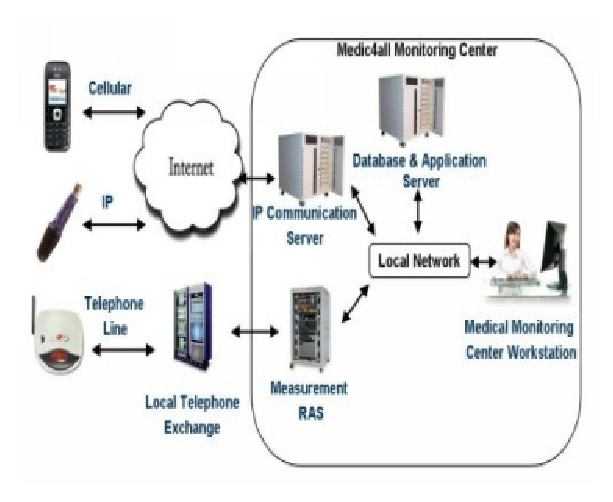
\includegraphics[width=100mm,keepaspectratio]{telcomed.eps}
\caption{A Telcomed rendszer �ttekint�se}\label{fig:telcomed}
\end{figure}

\subsection{Keretrendszerek}

Egy �letviteli rendszer sz�mos csom�pontb�l �s v�gpontb�l �ll. A
v�gpontok inform�ci�t fogadhatnak ha riaszt�s �rkezik, valamint
d�nt�shozatal vagy szenzorok eset�n inform�ci�t k�ldhetnek is. A
rendszer l�trehoz�sakor a legt�bb probl�ma m�r itt jelentkezik: a
v�gpontokat valamilyen m�don a csatlakoz�si pontokhoz kell k�tni, erre
nem volna h�tr�nyos valamilyen szabv�nyos megold�st haszn�lni, valamint
el szeretn�nk ker�lni a ker�k feltal�l�s�t is.

Ebb�l k�vetkezik, hogy a rendszert mindenk�ppen �rdemes valamilyen
jelenleg is el�rhet� keretrendszerre �p�teni, �s nem teljesen �n�ll�
egys�gk�nt l�trehozni.

E bevezet� alfejezet c�lja ismertetni ezek k�z�l n�h�ny jelenleg is
haszn�latban l�v� megold�st, hogy ezek ut�n legyen viszony�t�si alapunk
az Erlang k�rnyezet �ltal ny�jtott funkcionalit�s meg�t�l�s�hez.

\subsubsection*{RPC}

Az egyik legels�\cite{rpc1} ilyen megold�st a Sun c�g specifik�lta ki
1988-ban. A szabv�nyt ma is akt�van haszn�lj�k, (e munka �r�s�nak
pillanat�ban) legutols� verzi�j�t\cite{rpc2} 2009-ben adt�k ki. A
megc�lzott probl�ma a k�vetkez�: adott egy C f�ggv�ny, �s szeretn�nk azt
transzparens m�don megh�vni, de �gy, hogy az egy m�sik g�pen fusson le.
Teh�t a kliens oldalon kell egy csonk (stub), mely azonos interf�sszel
rendelkezik, mint az eredeti f�ggv�ny, de az implement�ci� mag�ban
foglalja a t�voli kiszolg�l�hoz val� csatlakoz�st, a t�voli k�dfuttat�st,
valamint az eredm�ny lek�r�s�t. A kiszolg�l� oldal�n szint�n sz�ks�g
van egy csonk f�ggv�nyre, mely lehet�v� teszi, hogy az RPC kiszolg�l�
k�r�s eset�n megh�vja a t�nyleges implement�ci�j�t a f�ggv�nynek. A
t�voli elj�r�sh�v�shoz egy interf�szt kell defini�lni egy
interf�sz-le�r� nyelvvel (Interface Description Language, IDL), majd
ebb�l a csonkok gener�lhat�ak p�ld�ul az \emph{rpcgen} programmal.

A m�dszernek manaps�g az egyik fontos felhaszn�l�si ter�lete a h�l�zati
f�jlrendszerek (Network File System, NFS). H�tr�nyai k�z�l legink�bb azt
�rdemes megeml�teni, hogy heterog�n k�rnyezetben, illetve nyitott
h�l�zaton limit�lt a funkcionalit�sa.

\subsubsection*{DCOM}

A DCOM\cite{dcom} (Distributed Component Object Model) technol�gi�t a
Microsoft alkotta meg, a szint�n �ltaluk kidolgozott COM (Component
Object Model) kiterjeszt�sek�nt. A DCOM nem titkolt sz�nd�ka
versenyt�rsk�nt megjelenni a k�s�bb eml�t�sre ker�l� CORBA
architekt�r�nak.

A DCOM m�g�tti gondolat az volt, hogy a n�pszer� COM technol�gi�t
tov�bbfejlessz�k, �s lehet�v� tegy�k az elj�r�sh�v�st t�voli
sz�m�t�g�pen is. A COM legfontosabb tulajdons�ga, hogy lehet�v� tette
alkalmaz�sok sz�m�ra, hogy egy publikus interf�szt defini�ljanak, �s az
ebben megjel�lt f�ggv�nyeket a g�pen fut� m�s alkalmaz�sok megh�vj�k. Az
RPC-hez k�pest �jdons�g, hogy az interf�szt nem kell el�re tudniuk a
klienseknek, hanem egy \texttt{QueryInterface()} f�ggv�nyen kereszt�l az
lek�rdezhet�.

Annak ellen�re, hogy alternat�v implement�ci�k el�rhet�ek m�s
rendszerekre is, ez a technol�gia igaz�n csak Windows rendszereken
terjedt el.

\subsubsection*{CORBA}

A CORBA\cite{corba} szabv�nyt az Object Management Group (OMG) dolgozta
ki, c�lja pedig, hogy t�bb nyelv, t�bb g�pen egy�tt tudjon m�k�dni,
teh�t lehet�v� tegye k�z�tt�k a t�voli elj�r�sh�v�st. Fontos �jdons�g
m�g benne, hogy teljes m�rt�kben hordozhat�.

Az interf�sz megad�sa itt is IDL seg�ts�g�vel t�rt�nik, viszont az is a
szabv�ny r�sze, hogy az IDL-t, hogyan kell lek�pezni sz�mos nyelvre.
Term�szetesen ezen k�v�l az el�re meghat�rozott nyelv-list�n k�v�l is
m�g t�bb nyelvhez el�rhet� a CORBA, de ott az implement�ci� m�r nem
szabv�nyos�tott.

A t�nyleges t�voli elj�r�sh�v�s k�t legfontosabb komponense itt a
objektum k�r�s br�ker (Object Request Broker, ORB -- az alkalmaz�s m�s
objektumokkal csak ezen kereszt�l l�phet interakci�ba), valamint az
objektum adapter (Object Adapter), amelynek feladata kezelni az
objektumok referencia-sz�ml�l�j�t, figyelni az �lettartalm�t, �s ehhez
hasonl� feladatokat ell�tni.

\subsubsection*{XML-RPC}

V�gezet�l megeml�tj�k az XML-RPC\cite{xmlrpc} szabv�nyt, mely HTTP
protokoll felett, XML haszn�lat�val oldja meg a t�voli elj�r�sh�v�st. Az
a megk�zel�t�s rendk�v�l n�pszer� napjainkban webszolg�ltat�sok eset�n,
valamint a Microsoft �ltal a DCOM lev�lt�s�ra megalkotott WCF (Windows
Communications Framework) is bel�l XML-RPC-t haszn�l.


\section{Egy-egy kiv�lasztott rendszer r�szletes ismertet�se}

\subsection{A Tunstall �letviteli rendszer}

A sz�mos, jelenleg el�rhet� �letviteli rendszer k�z�l az angol Tunstall
c�g �letviteli rendszer�t v�lasztottuk r�szletesebb ismertet�s c�lj�b�l.
Ennek oka, hogy az �ltaluk ny�jtott szolg�ltat�sokr�l r�szletes
inform�ci�t tettek el�rhet�v�, valamint sz�mokkal, val�s �letb�l vett
p�ld�kkal �s esettanulm�nyokkal szolg�lnak az �rdekl�d�nek, �gy engedve
betekint�st b�rmely ak�r nem kompetens �rdekl�d�nek is.

\begin{figure}[htp]
\centering
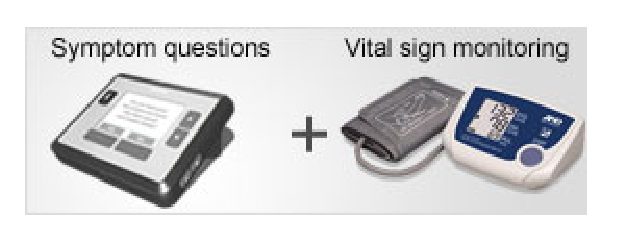
\includegraphics[width=75mm,keepaspectratio]{tunstall.eps}
\caption{A Tunstall Telehealth Monitor egy Bluetooth alap� v�rnyom�sm�r�vel}\label{fig:tunstall}
\end{figure}

A c�g �ltal l�trehozott �letviteli rendszer sz�mos, a napi �letben
el�fordul� probl�m�t igyekszik megoldani:

\begin{itemize}
	\item Elmezavar. Gyakori probl�ma, hogy az ilyen probl�m�kkal
k�zd� emberek elhagyj�k otthonukat, majd indokolatlanul sok ideig nem
t�rnek vissza. A c�g forgalmaz olyan szenzort, amely adott id�
eltelt�vel riaszt, ha nem t�rt�nt meg a haza�rkez�s. Egy hasonl�
probl�ma, hogy az �gyb�l kikelve nem tal�lj�k az utat a f�rd�szoba fel�,
vagy vissza, ehhez is l�trehoztak egy megold�st, mely �rz�keli, hogy
mikor kelt ki az �gyb�l az ember, �s ekkor kapcsolja be a vil�g�t�st az
�tvonal k�nnyebb megtal�l�s�hoz. V�g�l az ilyen emberek sokszor
k�ptelenek felm�rni, hogyha vesz�lybe keveredtek, �s nem teszik meg a
sz�ks�ges �vint�zked�seket. A c�l f�st-, sz�ndioxid- �s
f�ldg�z-�rz�kel�ket is forgalmaz, melyek egy k�zpontban riasztanak, ha
seg�ts�gre van sz�ks�g.
	\item Es�sek. Naponta 8000 id�sebb vagy gyenge ember esik el.
\footnote{Ez, �s a t�bbi sz�m a Tunstall c�g �ltal, a jelen �r�s
pillanat�ban (2009 okt�ber) k�z�lt adatokb�l val�, �s Angli�ra
vonatkozik.}
Ezek 70 sz�zal�ka �jszaka t�rt�nik. Minden �t�dik ember, aki elt�ri a
cs�p�j�t 6 h�napon bel�l hal meg. Ebb�l k�vetkezik, hogy ha egy embernek
f�lnie kell az eles�st�l, az mag�val vonja azt az �rz�st, hogy m�r nem
k�pes f�ggetlen�l mozogni, valamint hogy m�r nem �l teljes �letet. A c�g
�gy k�t probl�mak�rt c�loz meg: egyr�szt minim�lisra cs�kkenteni az
es�sek hat�s�t, m�sr�szt n�velni az indokolatlanul kis m�rt�k�
�nbizalmat. A c�g olyan szenzort forgalmaz, mely �rz�keli, ha az ember
elhagyta az �gy�t, �s nem t�rt vissza meghat�rozott id�n bel�l, ami
v�lhet�leg arra utal, hogy az illet� elesett. Az es�s-�rz�kel� egy
der�ksz�jon viselt szenzor, mely egyr�szt automatikusan �rz�kelni k�pes
az es�st, valamint egyszer� megold�st ad az elesett ember sz�m�ra is az
es�s jelz�s�re, �gy a gyors seg�ts�g ny�jt�sa k�nnyebb� v�lik. A
harmadik m�szer pedig egy mozg�s-�rz�kel�, mely akkor riaszt, ha az
ember hosszabb ideje nem mozgott m�g lak�son bel�l, mely nagy
val�sz�n�s�ggel eles�st jelent. Ezek az eszk�z�k seg�tenek megel�zni
olyan eseteket, mikor p�ld�ul egy id�s ember a f�rd�szob�b�l visszat�rve
elesik a k�sz�b�n, majd az eg�sz �jszak�t ott kell t�ltse, mivel nem tud
seg�ts�get k�rni.
	\item �tmeneti biztos�t�s. Ennek c�lja, hogy olyan emberek akik
kis seg�ts�ggel m�r otthon gy�gyulhatn�nak, sokszor a k�rh�zban
maradnak, �s ott lassabban gy�gyulnak, csup�n n�h�ny k�nnyen
kik�sz�b�lhet� probl�ma miatt. Ilyen p�ld�ul az el�z� pontban eml�tett
es�s-�rz�kel�, e n�lk�l egy l�badoz� beteget hazaengedni felel�tlens�g
lenne.
	\item Tanul�si neh�zs�gek. Hetente 200 ember sz�letik tanul�si
neh�zs�gekkel. Ez azt jelenti, hogy �j vagy �sszetett inform�ci�kat,
�n�ll�s�got az �tlagos embern�l nehezebben tanulnak. A c�g c�lja, hogy
ezeknek az embereknek a tanul�si neh�zs�gein seg�tve ne ker�ljenek t�vol
a csal�djukt�l, vagy valamilyen k�z�ss�g r�szek�nt �n�ll�bb �letet
tudjanak �lni.

P�ldak�nt lehetne eml�teni az el�z� pontokban is r�szletezett szenzort,
mely az �gy elhagy�sakor �s adott id�n bel�l val� vissza nem t�r�skor
jelez, �gy �rtes�tve a csal�dtagokat, ha probl�ma mer�lt fel, m�g az
esetek nagy r�sz�ben a rokonok nyugodtan alhatnak, hiszen a szenzor
jelz�s�re biztosan fel�brednek.
\end{itemize}

A technikai r�szletekr�l kevesebbet lehet tudni, de az�rt akadnak kiv�telek. A
British Telecom\cite{bt} angol telefont�rsas�ggal egy�ttm�k�dve sz�mos
IP-alap� szolg�ltat�st tettek el�rhet�v�. A BT 21 CN\cite{bt21cn} (21st
Century Network) n�ven elind�tott programjuk technikai szempontb�l
legink�bb a hagyom�nyos telefonh�l�zat (PSTN) lecser�l�se VoIP
megold�sokra. Ez lehet�v� teszi, hogy az egyes v�gpontokon ne csak
besz�det, hanem sokf�le adatforgalmat is lebonyol�tsanak az �gyfelek. Ez
a megold�s kiv�l�an haszn�lhat� a szenzorok �ltal gy�jt�tt adatok
tov�bb�t�s�ra, valamint sz�ks�g eset�n riaszt�sra. A Tunstall egy list�t
vezet azokr�l a szenzorokr�l, melyek a 21CN h�l�zat felett haszn�lt,
�ltaluk bevezetett protokollt t�mogatni tudj�k. Sajn�latos m�don azonban
nem �rhet� el r�szletes inform�ci� az �ltaluk kifejlesztett, �s �les
�zemben is haszn�lt protokoll r�szleteir�l.

\subsection{Az OSGi keretrendszer}

Az OSGI Sz�vet�g (r�gebbi nev�n Open Services Gateway initiative) egy
ny�lt szabv�ny�gyi szervezet. A sz�vets�g tagjai egy Java-alap�
szolg�ltat�s-platformot defini�ltak, mely t�volr�l kezelhet�.

A szabv�ny m�g�tt olyan neves c�gek �llnak, mint a Nokia, Motorola vagy
az IBM. Legink�bb mobil eszk�z�kben haszn�lj�k, de p�ld�ul a n�pszer�
Eclipse IDE is ezt haszn�lja a be�p�l� moduljainak kezel�s�re.  A
szabv�ny sz�t itt a hagyom�nyos �rtelemben haszn�lhatjuk, mivel csak a
ny�lt forr�s� implement�ci�kat sz�molva is t�bbessz�mr�l besz�lhet�nk.

\begin{figure}[htp]
\centering
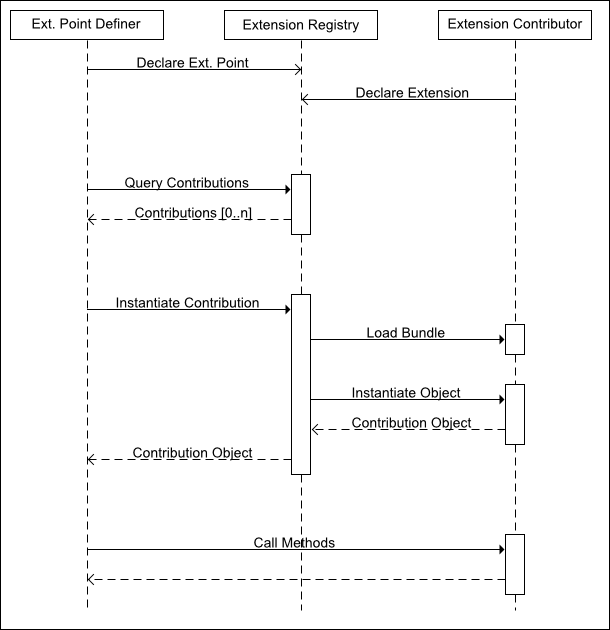
\includegraphics[width=100mm,keepaspectratio]{extensions.eps}
\caption{UML szekvenciadiagram, mely Eclipse kiterjeszt�sek m�k�d�s�t mutatja be, mely OSGi-t haszn�l.}\label{fig:extensions}
\end{figure}

El�sz�r 2000-ben jelent meg, a jelenleg aktu�lis 4-es verzi�j�t pedig
2009 szeptember�ben adt�k ki, �gy m�lt�n tekinthet�nk r�, mint akt�van
fejlesztett �s karbantartott megold�sra.

A keretrendszer legfontosabb elemei:

\begin{itemize}
	\item Alkalmaz�sok �letciklus�nak kezel�si modellje: az
alkalmaz�sokat csomagok (bundle) form�j�ban lehet terjeszteni, majd a JVM
le�ll�t�sa n�lk�l telep�teni, elind�tani, friss�teni vagy elt�vol�tani.
	\item Szolg�ltat�s adatb�zis: ez az adatb�zis lehet�v� teszi az
alkalmaz�sok sz�m�ra, hogy �rtes�ljenek ha �j szolg�ltat�sok �rhet�ek el
vagy egy szolg�ltat�s megsz�nt, �s �gy alkalmazkodhatnak az �j
k�rnyezethez.
	\item V�grehajt�si k�rnyezet: A v�grehajt�si k�rnyezet azt
defini�lja, hogy egy k�rnyezetben milyen oszt�lyok �s met�dusok �rhet�ek
el. A Java Platform, Standard Edition is egy elfogadott OSGi
v�grehajt�si k�rnyezet, de a CDC keretrendszer (amit p�ld�ul a legt�bb
mai mobiltelefon is t�mogat) is t�mogatott, valamint van saj�t, �ltaluk
defini�lt k�rnyezet is. Minden egyes OSGi implement�ci� maga d�ntheti
el, hogy milyen v�grehajt�si k�rnyezetet t�mogat, az el�bbieket a
legt�bb t�mogatja.
	\item Modulok: Azt is szabv�nyos�tott�k, hogy az egyes csomagok
milyen m�don tudj�k az egym�s k�zt fenn�ll� f�gg�s�geket, valamint a
k�v�lr�l el�rhet� API-kat defini�lni, lehet�v� t�ve ez�ltal, hogy
egys�ges m�don lehessen az egyes egys�gekb�l �s egys�gekbe
met�dus-h�v�sokat v�gezni.
\end{itemize}

\begin{figure}[htp]
\centering
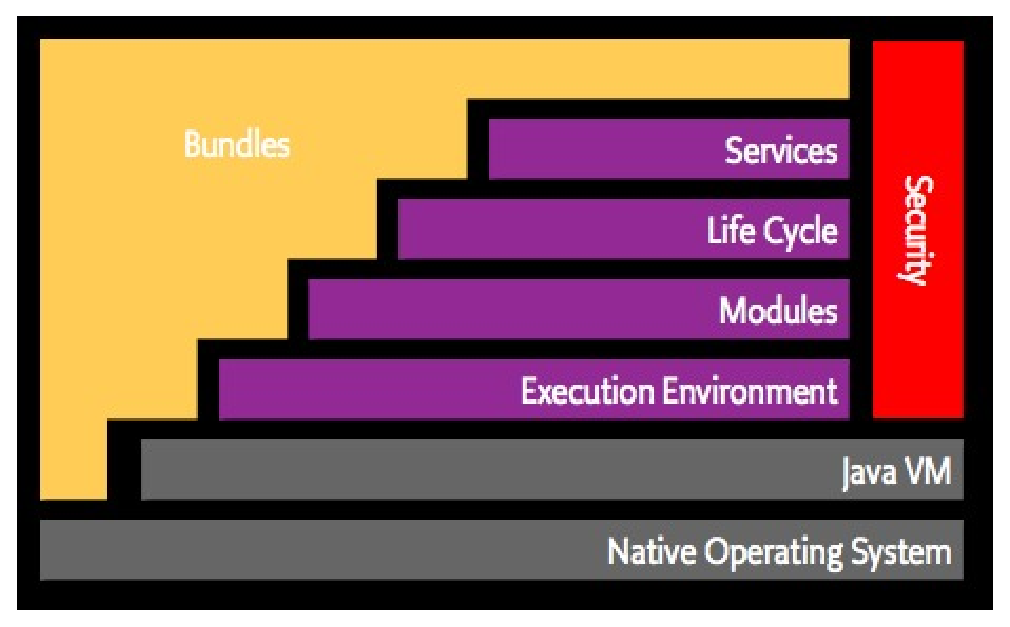
\includegraphics[width=100mm,keepaspectratio]{layering-osgi.eps}
\caption{Az OSGi r�tegei}\label{fig:layering-osgi}
\end{figure}

Az egyes csomagok olyan Java k�nyvt�rak (JAR f�jlok), amik
OSGi-specifikus fejl�ccel rendelkeznek a JAR MANIFEST.MF f�jlj�ban.

Az egyes alkalmaz�soknak a k�vetkez� �llapotai lehetnek:

\begin{itemize}
	\item Telep�tve: Ekkor m�g elk�pzelhet�, hogy egy csomag
f�gg�s�gei nem �llnak rendelkez�sre.
	\item Feloldva: Minden f�gg�s�g el�rhet�, az alkalmaz�st vagy
le�ll�tott�k, vagy k�sz az indul�sra.
	\item Indul: Az alkalmaz�s aszinkron m�don el lett ind�tva, de
m�g nem t�rt vissza.
	\item Akt�v: Az alkalmaz�s elindult, �s m�g nem kezdem�nyezt�k a
le�ll�t�s�t.
	\item Le�ll: Az alkalmaz�s le�ll�t�sa aszinkron m�don
elkezd�d�tt, de m�g nem fejez�d�tt be.
	\item Elt�vol�tva: Az alkalmaz�s �jabb telep�t�sig nem ind�that�
el.
\end{itemize}

A szolg�ltat�sok Java interf�szeket jelentenek. Ezeket az API-kat
implement�lhatj�k a csomagok, majd ha a csomagot regisztr�lt�k  a
szolg�ltat�s-adatb�zisban, akkor a kliensek itt megtal�lhatj�k �ket, �s
innent�l �rtes�t�st k�rhetnek a szolg�ltat�s el�rhet�s�ge �s el nem
�rhet�s�ge eset�n.

Az OSGi szabv�ny is tartalmaz el�re defini�lt szolg�ltat�sokat, melyeket
h�rom csoportra oszthatunk:

\begin{itemize}
	\item OSGi System Services: ide tartoznak az olyan
rendszerszolg�ltat�sok, mint az esem�nykezel�, a be�ll�t�skezel�,
alkalmaz�sok adminisztr�ci�ja, I/O m�veletek, felhaszn�l�kezel�s.
	\item OSGi Protocol Services: El�re defini�lt protokollok
haszn�lat�t seg�ti -- HTTP feletti kommunik�ci�t, UPnP-t t�mogat� �s
mobil eszk�z�k fel� val� kommunik�ci�t.
	\item OSGi Miscellaneous Services: Ide tartozik minden egy�b
el�re defini�lt szolg�ltat�s, p�ld�ul XML �rtelmez�.
\end{itemize}


\section{Az Erlang-alap� �letviteli rendszer terve}

Az �ltalunk tervezett �letviteli rendszer legfontosabb ism�rve teh�t az
lesz, hogy Erlang k�rnyezetben val�s�tjuk meg. Ezen fejezet c�lja
specifik�lni a k�vetelm�nyrendszert, �s e specifik�ci� n�h�ny
jellegzetes elem�t fogjuk megval�s�tani a k�vetkez� fejezetben.

\subsection{F� k�vetelm�nyek}

\subsubsection{Elosztotts�g}

Elosztott rendszert tervez�nk, ez a jelen esetben azt jelenti, hogy
nincs k�zponti eleme a rendszernek, �s ez �ltal nincsen egyetlen olyan
elem sem, amelynek a meghib�sod�sa eset�n az eg�sz rendszer le�llna. Egy
egyszer� p�lda: az id�s ember elhagyja az �gy�t, majd a lak�s�t is, �s
megadott id�n bel�l nem t�r vissza. K�t szenzor is jelez a t�relmi id�
letelte ut�n. A rendszer lehet�s�get ad arra, hogy egy szenzor t�bb
k�zpontnak is jelezzen, valamint azt, is, hogy egy k�zpontban ugyanarr�l
a jelz�sr�l t�bben is �rtes�t�st kapjanak. Term�szetesen a redundanci�t
tov�bb is fokozhatjuk, de ha ezt nem is tessz�k, akkor is a k�vetkez�kre
sz�m�thatunk:

\begin{itemize}
\item Legrosszabb esetben is kieshet egy elem, �s a rendszer�nk
t�k�letesen fog tov�bb �zemelni.
\item K�t elem kies�sekor m�r fenn�ll a vesz�lye annak, hogy gond lesz,
p�ld�ul ha a k�t szenzor esik ki.
\item Legjobb esetben h�rom elem is kieshet: ha pont az egyik szenzor,
az egyik k�zpont �s az egyik termin�l esik ki.
\end{itemize}

A redundanci�n, mint az �letviteli rendszerek szempontj�b�l a legink�bb
szembet�n� el�ny�n k�v�l azonban m�s pozit�vumai is lehetnek egy
elosztott rendszernek. Eml�t�sre m�lt�, hogy a termin�lok ak�r
lev�lasztott (h�l�zati kapcsolat n�lk�li) �llapotban is hozz�f�rnek a
kor�bban megkapott �zenetekhez, valamint ha ezek k�z�tt keresni akarnak,
az szint�n gyorsabb lesz, mint egy k�zpontos�tott rendszer eset�n,
hiszen nem kell h�l�zati k�sleltet�ssel sz�molni.

\subsubsection{A rendszer elemei}

\paragraph*{Csom�pontok}

Elosztott rendszer l�v�n a rendszer \emph{csom�pontokb�l} �p�l fel. A
csom�pontoknak k�t fontosabb fajt�j�t k�l�nb�ztetj�k meg: a
\emph{k�zpontokat} �s a \emph{v�gpontokat}.

\paragraph*{K�zpontok}

Egy k�zpont bekapcsol�s ut�n nem tesz semmit, csak v�r arra, hogy
v�gpontok keress�k. Ha egy v�gpont k�zpontot keres, akkor v�laszol. Ha
egy v�gpont regisztr�l, akkor nevet ad neki, �s erre a n�vre m�s
v�gpontok feliratkozhatnak. Ilyen m�don a v�gpont �gy k�ldhet �zenetet,
hogy nem tudja, pontosan ki fogja megkapni. T�nylegesen csak a
k�zpontnak k�ldi el, majd a k�zpont k�ldi tov�bb a feliratkozott
v�gpontoknak.

A k�zpont nem rejti el az eredeti felad�t, az �zenetet kapott v�gpontnak
lehet�s�ge van v�laszolni az eredeti felad�nak, ha
p�ld�ul d�nt�s sz�ks�ges. Ebben az esetben az �zenet k�zvetlen�l ker�l
�tvitelre a k�t v�gpont k�z�tt, k�zpontok ig�nybev�tele n�lk�l.

A k�zpont ezenk�v�l hajland� kiadni egy n�v m�g�tt �ll� szenzor c�m�t
is, ez akkor hasznos, hogyha a v�gpont tudja a sz�m�ra �rdekes szenzor
nev�t, de az aktu�lis c�m�t nem, valamint a szenzor sose ad ki mag�r�l
adatot implicit m�don, �gy m�s m�don a v�gpont nem szerezhetne tudom�st
a szenzor c�m�r�l.

\paragraph*{V�gpontok}
A v�gpontok bekapcsol�s ut�n sz�rt �zenetet k�ldenek, majd v�rnak, am�g
legal�bb egy k�zpont v�laszol a k�r�sre.  A v�gpontoknak k�t fajt�j�t
k�l�nb�ztetj�k meg. Ezek egym�st�l sokkal ink�bb logikailag, mintsem
technikailag k�l�nb�znek.

\paragraph*{Szenzorok}
A \emph{szenzorok} olyan �rz�kel�k, melyek a k�rnyezetr�l szolg�ltatnak
inform�ci�t. Ez az inform�ci�-ad�s lehet implicit vagy explicit.
Implicit esetben azt �rtj�k, ha p�ld�ul egy h�m�r� a m�rt
h�m�rs�kletet �r�nk�nt elk�ldi az �ltala ismert k�zpontoknak. Explicit
esetben viszont egy m�sik v�gpont k�r�s�re, k�zvetlen�l a m�sik
v�gpontnak b�rmikor elk�ldheti a k�rt adatot. L�thatjuk, hogy az
implicit esetet nem el�zi meg k�r�s-�zenet, m�g explicit esetben mindig
csak egy v�gpont kap �rtes�t�st.

Egy �rdekes probl�ma annak a jelens�gnek a kezel�se, mely olyan
szenzorok integr�l�sakor mer�l fel, melyek folyamatosan m�rnek. Ezeket
nem lehet explicit m�don lek�rdezni, viszont az �sszes m�rt adat
implicit k�zl�se indokolatlanul nagy h�l�zati forgalmat �s adatmennyis�get gener�lna. Ezt a
probl�m�t �gy k�sz�b�lhetj�k ki -- ez�ltal ezt a szenzor-t�pust
beillesztve a fenti k�t szenzor-kateg�ri�ba --, hogy a m�szer el�
tesz�nk egy modult, mely mindig t�rolja az utolj�ra m�rt �rt�ket. �gy a
legut�bbi m�rt adat explicit m�don b�rkinek b�rmilyen id�pontban
el�rhet�v� v�lik.

Egy m�sik tulajdons�g, melyben a szenzorok k�l�nb�zhetnek, a
vez�relhet�s�g.

P�ld�ul egy h�m�r� eset�ben a legt�bbsz�r nincs mit vez�relni, ellenben
egy h�z ajtaj�ba szerelt z�r eset�n megoldhat�, hogy ne csak lek�rdezni
tudjuk, hanem a z�r �llapot�t vez�relni is lehessen.

\paragraph{Termin�lok}
A \emph{termin�lok} olyan v�gpontok, melyek els�sorban �zenetek
fogad�s�ra hivatottak, teh�t bekapcsol�s ut�n keresnek legal�bb egy
k�zpontot, valamint vagy el�re be�ll�tott, vagy a felhaszn�l� �ltal
interakt�van be�ll�that� m�don feliratkoznak a k�zpont(ok)
n�vszolg�ltat�sa �ltal adott esem�nyekre. A termin�l lehet
passz�v, mint p�ld�ul egy k�perny�, vagy akt�v, p�ld�ul egy
mobiltelefon. Az akt�v termin�lok reag�lhatnak egy-egy �zenetre, m�g a
passz�vok csak t�j�koztat� �zeneteket k�pesek megjelen�teni.

Egy lehets�ges szcen�ri� p�ld�ul a k�vetkez�: a t�zjelz� jelez a k�zpontnak, a
k�zpont tov�bb�tja az �zenetet egy telefonra, ott a c�lszem�ly egy
�zenetet k�ld a t�zjelz�t tartalmaz� lak�s ajtaj�ban l�v� z�rnak, hogy
az adja meg az �llapot�t, az v�laszol k�zvetlen�l a telefonra, hogy
z�rva van, majd a c�lszem�ly �gy d�nt, hogy ez az �llapot nem k�v�natos,
�s egy olyan vez�rl�-�zenetet k�ld a z�rnak, hogy az ny�ljon ki. Ez a
folyamat ak�r meg is mentheti egy id�s ember �let�t, aki nem k�pes a
nagy f�stben kinyitni a z�rat, ellenben az egyszer�en kilinccsel
nyithat� ajt�n kereszt�l m�r k�pes elhagyni a lak�st.

\subsubsection{Dinamizmus}

Volt m�r sz� arr�l, hogy minden csom�pont fut�si id�ben
k�pes v�ltoztatni azon csom�pontok list�j�t, amelyekkel kommunik�lni
k�pes. K�zpontok eset�n ez azt jelenti, hogy egy �j szenzor
regisztr�ci�jakor nem kell a rendszert �jraind�tani, a v�gpontok pedig
b�rmikor lek�rhetik egy �zenetb�l az eredeti felad�t, vagy egy k�zpont
n�vszolg�ltat�s�n kereszt�l egy, a n�v m�g�tt �ll� szenzor c�m�t, majd
annak �zenetet k�ldhetnek. Ezek az ig�nyek n�lk�l�zhetetlenek a rendszer
m�k�d�s�hez.

Amire viszont els� k�rben nem biztos, hogy gondoln�nk, az az, hogy a
k�zpontoknak k�l�nb�z� t�pus� szenzorokat kell kezelni�k, �s ez
kor�ntsem egyszer� feladat. A probl�ma az, hogy minden szenzor m�s m�don
hajland� adatokat szolg�ltatni. M�g ha felt�telezz�k is, hogy minden
szenzor egyben Erlang csom�pont is, akkor is m�s �zenetet kell k�ldeni egy
h�m�r�nek (p�ld�ul \texttt{getTermperature()}), �s m�st egy
v�rnyom�sm�r�nek (p�ld�ul \texttt{getBloodPressure()}). Ezek egys�ges
kezel�s�hez a k�zpontban meghajt�programok sz�ks�gesek.

A megold�s az, hogy minden szenzort�pus egyedi
azonos�t�val rendelkezik, ezt elk�ldi a k�zpontnak, a k�zpont az
azonos�t� alapj�n let�lt egy meghajt�programot, bet�lti, �s onnant�l tudja, hogy
hogyan kell kezelni.

\subsubsection{Biztons�g}

Az el�z� alfejezet c�m�r�l, a dinamizmus sz�r�l m�g egy jelens�g
juthat esz�nkbe: am�g m�k�dik, addig j�, de ha valami gond van a
rendszerrel, akkor bajban vagyunk, hiszen egy dinamikusan m�k�d�
rendszerben hib�t keresni nem kellemes feladat. Ha tov�bb keress�k a
probl�m�kat a dinamizmussal, akkor felmer�l az a k�rd�s is, hogy milyen
biztons�gi kock�zatokat hozunk be ezzel a rendszerbe.

A k�t probl�ma l�tsz�lag �sszef�gg, de val�j�ban f�ggetlen. Az intelligens,
plug-and-play rendszerekre val�s ig�ny van, k�l�n�sen id�s emberek eset�ben, hiszen �k
nem szakemberek, �gy nem v�rhat� el, hogy hosszabb tanul�s el�zi meg a
rendszer haszn�lat�t. Tekintve, hogy els�sorban ��rt�k j�n l�tre a
rendszer, ezt nem hagyhatjuk figyelmen k�v�l. A m�sik c�l -- a rendszer
�zemeltet�inek szemsz�g�b�l -- term�szetesen az, hogy min�l ink�bb kontroll
alatt legyen a rendszer, manu�lisan be�ll�tva a param�tereket, hogy a nem v�rt
viselked�st elker�lj�k. Sajnos a k�t c�lt nem lehet kifog�stalanul
teljes�teni egyszerre, de tal�lhatunk olyan kompromisszumos megold�st,
mely mindk�t f�l t�r�shat�r�n bel�l helyezkedik el.

A biztons�g k�rd�se annyiban kapcsol�dik az el�z� probl�m�hoz, hogy egy
biztons�gos rendszer egyik alapfelt�tele, hogy minden, a rendszer
sz�m�ra �rdekes objektum azonos�tva legyen, ami jelen esetben azt
jelenten�, hogy a felhaszn�l�k �s az eszk�z�k is valamilyen
autentik�ci�s mechanizmus teljes�t�se ut�n v�lhassanak csak a rendszer
r�sz�v�. Ez probl�m�t jelenthet p�ld�ul egy id�s embern�l, aki
telefon�lni se tud, mikor elesett, nemhogy jelszavakat megadni, miel�tt
�rtes�ten� a k�zpontot. Ezzel ellent�tes ig�ny, hogy ne helyezhessen el
b�rki egy termin�lt az ablakunk alatt, mely azonnal �rtes�ti a t�mad�t,
ahogy elhagytuk a lak�st.

Jelen munk�ban ezt a felmer�l� k�t probl�m�t �gy oldjuk meg, hogy
felt�telezz�k a k�zvetkez�ket:

\begin{itemize}
	\item A k�zpontoknak van interakt�v felhaszn�l�i fel�lete.
	\item A k�zpontokhoz fizikailag csak olyan szem�ly f�r hozz�,
akinek van is jogosults�ga ehhez.
	\item A rendszer minden v�gpontja egyedi azonos�t�val
rendelkezik, melyet nem tud megv�ltoztatni.
	\item A kommunik�ci�ra haszn�lt csatorna biztons�gos. (Vagy
titkos�tott, vagy z�rt a h�l�zat.)
	\item Ha a k�zpontokhoz �j szenzor vagy termin�l pr�b�l
csatlakozni, akkor azt els� alkalommal a k�zpontban j�v� kell
hagyni. Legal�bb az els� v�gpont j�v�hagy�s�t fizikailag a k�zpontban
kell elv�gezni. (Innent�l az enged�lyezett eszk�z t�volr�l is
enged�lyezhet m�s eszk�z�ket.)
\end{itemize}

Ezekkel a felt�telekkel id�s emberek is k�nnyen integr�lhatnak �j,
gy�rilag a rendszerrel kompatibilisnek tervezett eszk�z�ket a
rendszerbe, an�lk�l, hogy potenci�lis biztons�gi r�seket hagyn�nk abban.

�sszehasonl�t�sk�ppen megeml�tj�k, hogy hasonl� jelleg� probl�ma mer�l
fel Bluetooth rendszerek eset�n, egy ,,�nlej�tsz�'' CD sz�m�t�g�pbe t�tele
eset�n, �s m�g sok m�s p�ld�t lehetne hozni. A Bluetooth rendszer eset�n
a megold�s az lett, hogy ha k�t eszk�z kommunik�lni akar, akkor azokat
egyszer p�ros�tani kell, �s ehhez a mechanizmushoz egy kor�bban
egyeztetett jelsz�t kell megadni. Ha mindk�t oldalon ugyanazt a jelsz�t
adj�k meg, akkor a p�ros�t�s siker�lt. Az CD-k eset�ben Windows
oper�ci�s rendszer eset�n �gy d�nt�ttek, hogy alap�rtelmez�sben
figyelmeztet�s n�lk�l elindul a program, amint behelyezt�k a CD-t a
meghajt�ba. Ezt term�szetesen tiltani lehet, �s a biztons�gi k�rd�sekre
kicsit komolyabban odafigyel� felhaszn�l�k ezt meg is teszik.
Ellenp�ldak�nt lehetne felhozni a legt�bb UNIX oper�ci�s rendszert, ahol
a CD automatikus csatol�sa vagy fel se mer�l probl�mak�nt, vagy a
felhaszn�l�bar�tabb rendszerekben is alap�rtelmez�sk�nt csak jelz�st
kap a felhaszn�l� a CD behelyez�s�r�l, de automatikus csatol�sra
felhaszn�l�i interakci� n�lk�l soha nem ker�l sor.

\subsubsection{Hat�rok}

A f� k�vetelm�nyek �ttekint�s�nek v�g�n megjegyezz�k azt, amire m�r a
bevezet�ben is utaltunk: jelen munka c�lja egy �letviteli rendszer
k�ztes r�teg�nek kidolgoz�sa. Sz�nd�kosan nem foglalkozunk teh�t a
k�vetkez�kkel:

\begin{itemize}
\item Sk�l�zhat�s�gi k�rd�sek. A rendszerben t�pusonk�nt kis sz�m�
elem tal�lhat� meg, kisebb finom�t�sok sz�ks�gesek lehetnek, ha a
rendszert t�pusonk�nt nagys�grendekkel t�bb elemmel haszn�ljuk, ezekre
nem t�r�nk ki.
\item Felhaszn�l�i fel�let. Az egyszer�s�g kedv��rt az �sszes
csom�pont a standard kimenetre (stdout) �rja az �zeneteit. Egy t�nyleges
rendszerben ezt c�lszer� valamilyen felhaszn�l�bar�tabb grafikus vagy
webes fel�letre cser�lni.
\item T�voli karbantart�s. A meghajt�k automatikus let�lt�s�n k�v�l egy�b
automatikus k�d-let�lt�ssel nem foglalkozunk, de megjegyezz�k, hogy a
meghajt�-let�lt�shez hasonl� m�don az egyes csom�pontok teljes szoftver�t
friss�thet�v� lehetne tenni. Az Erlang rendszer haszn�lata eset�n --
ahol fut�s k�zben lehet modulokat bet�lteni vagy friss�teni -- ehhez
nincs is sz�ks�g komolyabb er�fesz�t�sekre.
\end{itemize}

\subsection{Erlang �s UML}

A rendszer tervez�sekor form�lis jel�l�srendszerk�nt az UML (Unified
Modeling Language) jel�l�seit haszn�ljuk. Az UML els�sorban
objektumorient�lt rendszerek tervez�s�re k�sz�lt, m�g Joe Armstrong\cite{armstrong}
szerint az Erlang nem objektumorient�lt nyelv, �gy a
jel�l�srendszer nem haszn�lhat� magyar�zat n�lk�l.

An�lk�l, hogy �ltal�nos megfeleltet�st �ll�tan�nk fel az
objektumorient�lt nyelvek fogalmai �s az Erlang rendszerben el�rhet�
elemek k�z�tt, a jelen �letviteli rendszer tervez�se sor�n a
k�vetkez�ket felt�telezz�k:

\begin{itemize}
\item Az objektumok az Erlang rendszerben Erlang processzek lesznek.
\item Ha egy Erlang processz �zenetet kap, �s az �zenet t�pusa szerint az
�zenetre m�s-m�s m�don reag�l, azt megfeleltethetj�k az objektumok
met�dusainak.
\item Szekvenciadiagramok eset�n objektumok l�trehoz�s�n
\texttt{spawn()} h�v�sokat �rt�nk, met�dush�v�son pedig adott t�pus�
�zenet k�ld�s�t.
\item �llapotdiagramok eset�n az egyes Erlang processzek �letciklus�t
�rtj�k, hiszen az Erlangban nincsenek friss�thet� v�ltoz�k, hacsak nem
sz�molunk egy k�ls� adatb�zissal.
\end{itemize}

A k�vetkez� alfejezetekben teh�t az el�z� alfejezetben kifejtett f�
szempontokat pontos�tjuk, az UML jel�l�seit haszn�lva.

\subsection{Az elemek katal�gusa}

A rendszer teh�t a k�vetkez� elemekb�l fog �llni:

\begin{itemize}
\item Node: a rendszerben l�v� b�rmilyen csom�pont
\item Center: olyan csom�pont, mely k�zpont
\item Endpoint: olyan csom�pont, mely v�gpont
\item Sensor: olyan v�gpont, mely els�sorban �zeneteket k�ld
\item Terminal: olyan v�gpont, mely els�sorban �zeneteket fogad
\item Message: a csom�pontok k�z�tti �zenetek form�tum�t defini�lja
\item Driver: a let�lthet� eszk�zmeghajt�k interf�sz�t defini�lja
\end{itemize}

\subsection{Az elemek le�r�sa}

\subsubsection*{Node}

\begin{itemize}
\item Le�r�s:

Egy Erlang processzt jel�l, mely egyedi, nem megv�ltoztathat�
azonos�t�val rendelkezik.

\item V�ltoz�k:

Id -- Egyedi azonos�t�, mely nem v�ltoztathat� meg.

\item Szolg�ltat�sok:

ping() -- Egy pong atommal v�laszol, jelezve, hogy a processz fut.
\end{itemize}

\subsubsection*{Center}

\begin{itemize}
\item Le�r�s:

Olyan Node-ot jel�l, melybe regisztr�lhatnak szenzorok,
valamint a regisztr�lt nevekre feliratkozhatnak termin�lok. Csak
tov�bb�tja az �zeneteket, nem t�nyleges felad� vagy c�mzett.

\item V�ltoz�k:

Sensors -- Regisztr�lt szenzorok n�v-c�m p�rjait tartalmaz� lista.

Subscriptions -- Nevekre feliratkozott termin�lok n�v-c�m p�rjait
tartalmaz� lista.

\item Szolg�ltat�sok:

start() -- Center ind�t�sa.

stop() -- Center le�ll�t�sa.

reg(Address, Name) -- Sensor c�m�nek regisztr�l�sa n�vk�nt.

subscribe(Name, Address) -- N�vre feliratkoz�s egy Terminal adott c�m�vel.

lookup(Name) -- Sensor nev�nek felold�sa c�mre.

notify(Message) -- Message felad�sa tov�bb�t�s c�lj�b�l.
\end{itemize}

\subsubsection*{Endpoint}

\begin{itemize}
\item Le�r�s:

Olyan Node-ot jel�l, mely csak k�ld vagy fogad �zeneteket, nem tov�bb�t.

\item V�ltoz�k:

Messages -- Be�rkezett �zenetek list�ja.

\item Szolg�ltat�sok:

start(Config) -- Endpoint ind�t�sa adott be�ll�t�sokkal.

stop() -- Endpoint le�ll�t�sa.
\end{itemize}

\subsubsection*{Sensor}

\begin{itemize}
\item Le�r�s:

Olyan v�gpontot jel�l, mely a k�lvil�g valamely v�ltoz�s�nak hat�s�ra
�zenetet k�ld. T�mogathat m�g vez�rl�st, illetve explicit lek�rdez�st
is.

\item V�ltoz�k:

Centers -- Azon k�zpontok list�ja, melyeket �rtes�teni kell, ha v�ltozott
a k�rnyezet.

\item Szolg�ltat�sok:

query(Message) -- Lek�rdez egy adott funkci�t, �s a felad� c�m�re
megk�ldi.

control(Message) -- Be�ll�t egy adott funkci�t.
\end{itemize}

\subsubsection*{Terminal}

\begin{itemize}
\item Le�r�s:

Olyan v�gpontot jel�l, mely els�sorban �zenetek fogad�s�ra hivatott.
Opcion�lisan �zeneteket is lehet vele k�ldeni, v�laszk�nt egy kor�bban
egy szenzort�l kapott �zenetre.

\item V�ltoz�k:

Centers -- Azon k�zpontok list�ja, melyekre fel kell iratkozni indul�skor.

\item Szolg�ltat�sok:

notify(Message) -- �zenet �tad�sa a termin�l sz�m�ra.
\end{itemize}

\subsubsection*{Message}

\begin{itemize}
\item Le�r�s:

Egy Erlang ennest jel�l, mely az adat mellett tartalmazza az adat
t�pus�t, felad�j�t, c�mzettj�t, tov�bb�t�j�t.

\item V�ltoz�k:

Data -- Egy sz�m, a m�rt �rt�k vagy d�nt�s.

Description -- Ha a szenzor t�bb t�pus� �rt�ket is m�rne, ez mondja meg,
hogy melyik t�pust jel�li a Data mez�.

From -- A felad�t jel�li.

To -- A c�mzettet jel�li.

Receiver -- A k�zpontot jel�li.
\item Szolg�ltat�sok:

Nincsenek.
\end{itemize}

\subsubsection*{Driver}

\begin{itemize}
\item Le�r�s:

Egy Erlang f�ggv�nyt �r le, lehet�v� t�ve, hogy k�l�nb�z�
szenzorokat egys�ges interf�szen �t kezelj�nk. Az eszk�zmeghajt�nak megk�ldj�k, hogy
melyik Node h�nyadik funkci�j�t akarjuk lek�rdezni/vez�relni, majd az
megmondja a funkci� nev�t, amit m�r az eszk�z meg�rt.

P�ld�ul a \texttt{translate(sensor0@clevo.local, 0)} hat�s�ra az adott
meghajt� v�lasza lehet a \texttt{sugar}, mely egy v�rnyom�s- �s
v�rcukorm�r� eset�n a v�rcukor lek�rdez�s�t teszi lehet�v�.

\item V�ltoz�k:

Nincsenek.
\item Szolg�ltat�sok:

translate(Node, Number) -- Megad egy atomot, melyet met�dusn�vk�nt
haszn�lhatunk ha a szenzort explicit m�don akarjuk lek�rdezni.
\end{itemize}

\subsection{Statikus strukt�radiagram}

%A statikus strukt�radiagram \aref{fig:statikus-struktura-diagram}.
%�br�n a rendszer elemeir�l t�rolt adatokat, azok �sszef�gg�seit �s
%kapcsolatait mutatja.

\begin{figure}[H]
\centering
\includegraphics[width=150mm,keepaspectratio]{statikus-struktura-diagram.eps}
\caption{A rendszer statikus strukt�radiagramja}\label{fig:statikus-struktura-diagram}
\end{figure}

A statikus strukt�radiagram a rendszer elemeir�l t�rolt adatokat, azok
�sszef�gg�seit �s kapcsolatait mutatja.

\subsection{Szekvenciadiagramok}

\subsubsection*{K�zpont indul�sa}

\begin{figure}[H]
\centering
\includegraphics[width=50mm,keepaspectratio]{kozpont-indulasa.eps}
\caption{Szekvenciadiagram: k�zpont indul�sa}\label{fig:kozpont-indulasa}
\end{figure}

Az �br�n l�that�, hogy a k�zpontot mindig a felhaszn�l� helyezi �zembe,
�s a k�zpont bekapcsol�s ut�n bel�p a v�rakoz�si hurokba.

Ebb�l a helyzetb�l azt�n majd k�s�bb a regisztr�l� vagy riaszt�
szenzorok �s feliratkoz� termin�lok mozd�thatj�k ki.

\subsubsection*{Szenzor regisztr�ci�ja}

\begin{figure}[H]
\centering
\includegraphics[width=75mm,keepaspectratio]{szenzor-regisztracioja.eps}
\caption{Szekvenciadiagram: szenzor regisztr�ci�ja}\label{fig:szenzor-regisztracioja}
\end{figure}

Az �bra mutatja, hogy a szenzor bekapcsol�sakor m�r legal�bb egy
k�zpontnak bekapcsolt �llapotban kell lenni a rendszerben. Ekkor a
szenzor regisztr�l, majd a k�zpont elk�ldi a c�m�t, melyre a szenzor
jelezhet, ha az sz�ks�ges.

\subsubsection*{Termin�l regisztr�ci�ja}

\begin{figure}[H]
\centering
\includegraphics[width=75mm,keepaspectratio]{terminal-regisztracioja.eps}
\caption{Szekvenciadiagram: termin�l regisztr�ci�ja}\label{fig:terminal-regisztracioja}
\end{figure}

A termin�l regisztr�ci�ja eset�n is el�k�vetelm�ny legal�bb egy k�zpont
m�k�d�se, ahova feliratkozhat a termin�l, de itt a k�zpontnak nem kell
azonos�t�t k�ldenie, hiszen a termin�l nem fogja �rtes�teni a k�zpontot
esem�nyekr�l.

\subsubsection*{�zenetk�ld�s szenzorr�l}

\begin{figure}[H]
\centering
\includegraphics[width=100mm,keepaspectratio]{uzenetkuldes-szenzorrol.eps}
\caption{Szekvenciadiagram: �zenetk�ld�s szenzorr�l}\label{fig:uzenetkuldes-szenzorrol}
\end{figure}

Az �bra azt mutatja, hogy az �zenetk�ld�s akkor �rtelmes, ha egy k�zpont
bekapcsol�sa �s a szenzor regisztr�ci�ja ut�n legal�bb egy termin�l
feliratkozott az �zenetekre az �zenetk�ld�s el�tt. Ilyenkor a szenzor a
k�zpontot �rtes�ti, a k�zpont pedig a termin�lt.

\subsubsection*{�zenetk�ld�s szenzorr�l, redund�ns eset}

\begin{figure}[H]
\centering
\includegraphics[width=120mm,keepaspectratio]{uzenetkuldes-szenzorrol-redundans-eset.eps}
\caption{Szekvenciadiagram: �zenetk�ld�s szenzorr�l redund�ns esetben}\label{fig:uzenetkuldes-szenzorrol-redundans-eset}
\end{figure}

Az el�z� eset �ltal�nos�t�sa, ha t�bb szenzort, k�zpontot �s termin�lt
helyez�nk el a rendszerben. Az �bra k�t-k�t p�ld�ny kommunik�ci�j�t
mutatja be abban az esetben, ha olyan esem�ny k�vetkezik be, melynek
hat�s�ra mindk�t szenzor jelez.

\subsubsection*{Explicit lek�rdez�s termin�lr�l}

\begin{figure}[H]
\centering
\includegraphics[width=100mm,keepaspectratio]{explicit-lekerdezes-terminalrol.eps}
\caption{Szekvenciadiagram: explicit lek�rdez�s termin�lr�l}\label{fig:explicit-lekerdezes-terminalrol}
\end{figure}

Explicit lek�rdez�s eset�n a termin�l el�sz�r a k�zponthoz fordul a
szenzor c�m��rt, majd a c�m birtok�ban k�zvetlen�l a szenzornak k�ld
�zenetet az adatok lek�rdez�se c�lj�b�l.

\subsubsection*{Eszk�z enged�lyez�se}

\begin{figure}[H]
\centering
\includegraphics[width=100mm,keepaspectratio]{eszkoz-engedelyezese.eps}
\caption{Szekvenciadiagram: eszk�z enged�lyez�se}\label{fig:eszkoz-engedelyezese}
\end{figure}

Az eszk�z�k enged�lyez�se eset�n az �br�n l�that� m�don els� alkalommal,
ha egy szenzor regisztr�lni vagy egy termin�l feliratkozni akar, akkor a
felhaszn�l�nak azt egyszer enged�lyeznie kell.


\section{Megval�s�t�s}

A megval�s�t�s sor�n a tervez�s folyam�n elemzett haszn�lati eseteket
fogjuk sorra implement�lni. Terjedelmi okokb�l nem val�s�tjuk meg
a teljes funkcionalit�st, �gy c�lszer� mindj�rt az elej�n defini�lni,
hogy mely r�szletek eset�n alkalmazunk egyszer�s�t�seket, �s hol c�l a
teljes megval�s�t�s.

A tervez�s sor�n defini�lt oszt�lyok, az p�rhuzamoss�g, hibat�r�s �s
elosztotts�g t�mogat�sa a program r�sz�t k�pezik. Az elk�sz�t�s sor�n
nyomon fogjuk k�vetni, ahogy a tervez�s szakasz�ban le�rt haszn�lati
esetek sorra m�k�d�k�pess� v�lnak.

Amit nem vagy csak egyszer�s�tve val�s�tunk meg:

\begin{itemize}
\item A szenzorok nem automatikusan fedezik fel a k�zpontokat, hanem egy
konfigur�ci�s �llom�ny el�re defini�lja ezek list�j�t.
\item A kor�bban felvetett biztons�gi k�rd�sekkel nem foglalkozunk,
felt�telezz�k, hogy a rendszer z�rt, a rendszer elemei pedig
megb�zhat�ak.
\item Eltekint�nk a grafikus felhaszn�l�i fel�let l�trehoz�s�t�l,
egyszer� parancssoros interf�szt adunk a felhaszn�l�nak.
\end{itemize}

\subsection{Els�, m�r m�k�d� v�ltozat}

A legkisebb m�k�d� v�ltozata a rendszernek az az eset, mikor a
rendszerben egy szenzor, egy k�zpont �s egy termin�l van. Mivel ez lesz
minden k�s�bbi v�ltozat alapja, tekints�k �t t�zetesen a m�k�d�s�t. A
k�s�bbiekben csak az ehhez a v�ltozathoz k�pest eszk�z�lt m�dos�t�sokat
ismertetj�k.

E v�ltozat m�k�d�se sor�n a felhaszn�l� egy k�zpontot ind�t, majd egy
termin�lt, mely regisztr�l a k�zpontba, v�g�l egy szenzort, mely indul�s
ut�n azonnal �rtes�t�st k�ld. Ezt az �rtes�t�st kapja meg a k�zpont, majd
tov�bb�tja a termin�lnak.

\subsubsection*{K�zpont}

A k�zpont h�rom olyan f�ggv�nyt defini�l, mely a processz �letciklus�t
�rinti:

\begin{lstlisting}
start() -> register(center, spawn(fun() -> put(sensors, []), put(subscriptions, []), loop() end)).

stop() -> center ! stop.

ping() -> rpc({ping}).
\end{lstlisting}

A start/0 f�ggv�ny egy �j processzt ind�t az aktu�lis csom�ponton, mely
inicializ�lja a szenzorok �s feliratkoz�sok list�j�t, majd v�rakoz�
�llapotba ker�l, ld. k�s�bb.

A stop/0 f�ggv�ny ennek az �j processznek k�ld egy �zenetet, melynek hat�s�ra az le�ll.

A ping/0 f�ggv�ny kiz�r�lag hibakeres�si c�lokat szolg�l a lejjebb
ismertet�sre ker�l� rpc/1 f�ggv�ny felhaszn�l�s�val, lehet�v� t�ve, hogy
megvizsg�ljuk, hogy a k�zpont v�laszk�pes-e.

Tov�bbi n�gy f�ggv�ny pedig a k�zpont t�nyleges vez�rl�s�re szolg�l:

\begin{lstlisting}
reg(Address, Name) -> rpc({reg, Address, Name}).

lookup(Name) -> rpc({lookup, Name}).

subscribe(Name, Address) -> rpc({subscribe, Name, Address}).

notify(Message) -> rpc({notify, Message}).
\end{lstlisting}

L�thatjuk, hogy ezek mind a lenn ismertetett rpc/1 f�ggv�ny k�r� �p�tett
csomagol� f�ggv�nyek.

A csomagol� f�ggv�nyek �ltal h�vott rpc/1 f�ggv�ny a k�vetkez�:

\begin{lstlisting}
rpc(Q) ->
 center ! {self(), Q},
 receive
  {center, Reply} ->
   Reply
 end.
\end{lstlisting}

A f�ggv�ny a kor�bban center n�ven regisztr�lt
\footnote{Regisztr�ci�n �s regisztr�ci� t�rl�s�n itt az Erlang
rendszer register/2 �s unregister/1 f�ggv�nyeit �rtj�k, ami lehet�s�get
ad arra, hogy az aktu�lis csom�ponton Pid-ekhez atomokat rendelj�nk.
Ezek a regisztr�ci�k m�s csom�pontokr�l nem l�that�ak, a teljes rendszer
szintj�n nem egyediek, �s ezt ki is fogjuk haszn�lni.}
processznek k�ld egy k�t
elem� ennest, megk�ldve a saj�t c�m�t, valamint a t�nyleges adatokat,
majd a v�laszk�nt kapott �rt�kkel t�r vissza.

V�g�l a center n�ven regisztr�lt processz�nk f� f�ggv�nye a k�vetkez�:

\begin{lstlisting}
loop() ->
 receive
  {From, {ping}} ->
   From ! {center, pong},
   loop();
  {From, {reg, Address, Name}} ->
   io:format("[~p] reg(~p,~p)~n", [node(), Address, Name]),
   Sensors = get(sensors),
   put(sensors, [{Address, Name}| Sensors]),
   From ! {center, ok},
   loop();
  {From, {lookup, Name}} ->
   io:format("[~p] lookup(~p)~n", [node(), Name]),
   Sensors = get(sensors),
   A = [A || {A, N} <- Sensors, N =:= Name],
   From ! {center, {ok,A}},
   loop();
  {From, {subscribe, Name, Address}} ->
   io:format("[~p] subscribe(~p,~p)~n", [node(), Name, Address]),
   Subscriptions = get(subscriptions),
   put(subscriptions, [{Name, Address}| Subscriptions]),
   From ! {center, ok},
   loop();
  {From, {notify, Message}} ->
   io:format("[~p] notify(~p)~n", [node(), Message]),
   {Data, Description, Fro, To, _Receiver} = Message,
   lists:foreach(fun(I) -> rpc:call(I, terminal, notify, [{Data, Description, Fro, To, node()}]) end,
    [A || {N, A} <- get(subscriptions), N =:= To]),
   From ! {center, ok},
   loop();
  stop ->
   init:stop()
 end.
\end{lstlisting}

Az egyes be�rkez� �zenetekre teh�t a k�vetkez� v�laszokat adja:

\begin{itemize}
\item A ping atomra mindig pong atommal v�laszol.
\item A reg atomra a param�terk�nt kapott szenzor c�m�t �s nev�t
regisztr�lja a egy list�ba, melyet a process dictionary-ben t�rol (mely az Erlang futtat�rendszer r�sze), �gy
k�s�bb is lehet�v� v�lik a m�dos�t�sa.
\item A lookup atomra a param�terk�nt kapott n�vhez tartoz� szenzor
c�met adja vissza a sensors list�b�l.
\item A subscribe atomra a param�terk�nt kapott n�vhez elt�rolja a kapott c�met.
\item A notify atom eset�n egy �t elem� ennest (melynek elemeit a
tervez�s sor�n Message n�ven defini�ltuk) v�r param�terk�nt. Ebben
szerepel az, hogy milyen n�vre sz�l az �zenet. A k�zpont azoknak a
termin�loknak tov�bb�tja az �zenetet, amelyek ilyen n�vvel iratkoztak
fel, bele�rva saj�t mag�t mint tov�bb�t�t.
\item V�g�l a stop atomra le�ll�tja az aktu�lis Erlang csom�pontot.
\end{itemize}

A m�sik k�t elemmel ellent�tben itt megfigyelhet�, hogy a k�zpontnak
nincs konfigur�ci�s �llom�nya, valamint elind�t�sa ut�n nincs semmilyen
bek�vetkez� esem�ny.

\subsubsection*{Termin�l}

A strukt�ra diagramban l�thattuk, hogy a Center �s a Terminal is egy
Node, �gy itt is megtal�lhat� a processz �letciklus�val
kapcsolatos h�rom f�ggv�ny:

\begin{lstlisting}
start(ConfigFile) ->
 {ok, Config} = file:consult(ConfigFile),
 Centers = [ {C, E} || {center, C, E} <- Config],
 lists:foreach(fun({C, E}) -> rpc:call(C, center, subscribe, [E, node()]) end, Centers),
 register(terminal, spawn(fun() -> loop() end)).

stop() -> terminal ! stop.

ping() -> rpc({ping}).
\end{lstlisting}

A start/1 f�ggv�ny azonban itt egy konfigur�ci�s �llom�nyt v�r param�ter�l. Erre egy p�lda:

\begin{lstlisting}
{center, center0@clevo.local, event}.
\end{lstlisting}

A konfigur�ci�s �llom�ny szintaxis�ra az egyetlen megk�t�s az, hogy
minden egyes sorban egy Erlang termnek kell lennie, mivel ezt fogadja el
a file:consult/1 �rtelmez� f�ggv�ny. A fenti file-ban az egyetlen sor egy
k�zpontra val� feliratkoz�st defini�l, erre utal a center atom. Az ennes
m�sik k�t param�tere a k�zpont c�m�t
\footnote{
A k�vetkez�, tesztel�sr�l is sz�l� fejezetben l�tni fogjuk, hogy mi az
oka annak, hogy a c�m ebben a form�tumban lett megadva. �ltal�noss�gban
a c�m egy csom�pontot �s egy g�pet azonos�t� atomb�l �ll, a kukac
karakterrel �sszek�tve.
}
�s annak az esem�nynek a nev�t
defini�lja, melyre fel szeretn�nk iratkozni az adott k�zpontban.

Az ind�t�s sor�n teh�t �rtelmezz�k a be�ll�t�sokat, �s a k�r�snek
megfelel�en feliratkozunk a k�zpontokn�l, azok subscribe met�dus�t
megh�vva. Ha ez megt�rt�nt, �zenetre v�runk a lenn ismertet�sre ker�l�
loop/0 f�ggv�ny haszn�lat�val.

A stop/0 �s ping/0 feladata �s m�k�d�se m�s ismer�s, a center modulban
defini�ltakkal megegyez�.

A termin�lnak egyetlen, a modellben is l�tez� met�dusa a notify/1:

\begin{lstlisting}
notify(Message) -> rpc({notify, Message}).
\end{lstlisting}

A center:notify/1-hez hasonl� m�don ez is csak csomagol� f�ggv�ny az
rpc/1 k�r�.

A terminal modul marad�k r�sze a kor�bban hivatkozott rpc/1 �s loop/0
f�ggv�nyekb�l �ll:

\begin{lstlisting}
rpc(Q) ->
 terminal ! {self(), Q},
 receive
  {terminal, Reply} ->
   Reply
 end.

loop() ->
 receive
  {From, {ping}} ->
   From ! {terminal, pong},
   loop();
  {From, {notify, Message}} ->
   io:format("[~p] notify(~p)~n", [node(), Message]),
   From ! {terminal, ok},
   loop();
  stop ->
   init:stop()
 end.
\end{lstlisting}

Az rpc/1 feladata teh�t kommunik�lni a terminal n�ven regisztr�lt
processzel: az �zenetk�ld�s ut�n v�laszra v�rni, majd azzal
visszat�rni. A center modulhoz hasonl� m�don itt is az�rt van erre
sz�ks�g erre a csomagol�sra, mivel terminal n�ven m�s csom�ponton m�s
processzt �rhet�nk el.

A loop/0 f�ggv�ny pedig �zeneteket v�r:

\begin{itemize}
\item A ping �s stop atomok az �letciklus monitoroz�s�ra �s vez�rl�s�re
szolg�lnak a center modullal megegyez� m�don.
\item A notify atomra pedig a termin�l egyszer�en a standard kimenetre
k�ldi a kapott �zenet tartalm�t, nem t�l felhaszn�l�bar�t m�don.
\end{itemize}

\subsubsection*{Szenzor}

A sensor modul implement�ci�ja a start, stop �s ping met�dusokra:

\begin{lstlisting}
start(ConfigFile) ->
 Data = data,
 {ok, Config} = file:consult(ConfigFile),
 Centers = [ {C, E} || {center, C, E} <- Config],
 lists:foreach(fun({C, E}) ->
  rpc:call(C, center, reg, [node(), E]),
  Message = {Data, desc, node(), E, false},
  rpc:call(C, center, notify, [Message])
 end, Centers),
 register(sensor, spawn(fun() -> put(desc, Data), loop() end)).

stop() -> sensor ! stop.

ping() -> rpc({ping}).
\end{lstlisting}

L�thatjuk, hogy a start f�ggv�ny itt is haszn�l egy konfigur�ci�s
�llom�nyt, melynek azonos a form�tuma a szenzor�val. A feladata
term�szetesen m�s: itt azt adja meg, hogy melyik k�zpontnak milyen n�ven
kell elk�ldeni a m�r�si adatainkat.

Az els� v�ltozat teh�t r�gt�n indul�s ut�n k�ld egy �zenetet a
konfigur�ci�s �llom�nyban megadott k�zpontba, a megadott esem�nynevet
haszn�lva, mely arr�l fogja inform�lni a termin�lokat, hogy a desc
t�pus� m�r�si adat �rt�ke data.

A tervez�s sor�n a szenzorok explicit lek�rdez�s�nek ig�nye is
felmer�lt, az ehhez sz�ks�ges f�ggv�nyek:

\begin{lstlisting}
query_data(Message) -> rpc({query_data, Message}).

control(Message) -> rpc({control, Message}).

rpc(Q) ->
 sensor ! {self(), Q},
 receive
  {sensor, Reply} ->
   Reply
 end.
\end{lstlisting}

Az el�z�ekben megszokott m�don ezek is az rpc/1 f�ggv�nyt h�vj�k,
melynek m�k�d�si elve nem v�ltozott a kor�bbi k�t modulhoz k�pest.

A kor�bban hivatkozott loop/0 f�ggv�ny pedig a k�vetkez�:

\begin{lstlisting}
loop() ->
 receive
  {From, {ping}} ->
   From ! {sensor, pong},
   loop();
  {From, {query_data, {_Data, _Desc, Fro, _To, _Recv}}} ->
   rpc:call(Fro, terminal, notify, [{get(desc), desc, node(), Fro, false}]),
   From ! {sensor, ok},
   loop();
  {From, {control, {Data, _Desc, _Fro, _To, _Recv}}} ->
   put(desc, Data),
   From ! {sensor, ok},
   loop();
  stop ->
   init:stop()
 end.
\end{lstlisting}

\begin{itemize}
\item A ping �s stop atomok kezel�s�t m�r ismerj�k
\item A query\_data atom hat�s�ra a szenzor process dictionary-j�b�l lehet lek�rdezni.
\item A control atom seg�ts�g�vel pedig vez�relni lehet a szenzort.
\end{itemize}

\subsection{Redund�ns m�k�d�s}

A redund�ns m�k�d�s k�t szempontb�l k�l�nb�zik az el�z� alfejezetben
ismertetett v�ltozatt�l:

\begin{itemize}
\item A rendszer ind�t�sakor mindh�rom elemb�l k�t-k�t p�ld�nyt kell ind�tani.
\item A termin�lok �s szenzorok konfigur�ci�s �llom�ny�ban k�t-k�t
k�zpontot kell defini�lni.
\end{itemize}

Ez ut�bbit p�ld�ul a k�vetkez�k�ppen tehetj�k meg:

\begin{lstlisting}
{center, center0@clevo.local, event}.
{center, center1@clevo.local, event}.
\end{lstlisting}

\subsection{Eszk�zmeghajt�k t�mogat�sa}

Meghajt�programokra akkor van sz�ks�g�nk, ha egy �ltal�nos interf�szen
kereszt�l akarunk el�rni egy-egy eszk�zt, melynek a speci�lis jellemz�it
nem ismerj�k. Tegy�k fel, hogy egy szenzor t�bbf�le m�r�st is k�pes v�gezni,
�s ezeket sz�mozzuk.  A megval�s�tott p�lda eset�n a szenzor egy
querydesc/0 f�ggv�nnyel rendelkezik, a termin�l ezt szeretn� explicit
m�don lek�rdezni, de csak annyit tud, hogy ez a nulladik t�pus� m�r�si
funkci�ja az eszk�znek. A driver modul fog abban seg�teni, hogy a 0
alapj�n megkapja a querydesc atomot.

A modul egyetlen translate/2 f�ggv�nyt defini�l az interf�sz�ben:

\begin{lstlisting}
sub(Str,Old,New) ->
       RegExp = "\\Q"++Old++"\\E",
       re:replace(Str,RegExp,New,[multiline, {return, list}]).

translate(Node, Num) ->
       Module = sub(sub(atom_to_list(Node), "@", "_"), ".", "_"),
       compile:file(Module),
       Modulea = list_to_atom(Module),
       list_to_atom(Modulea:translate(Num)).
\end{lstlisting}

Az els� seg�df�ggv�ny csom�pont nev�b�l a modul nev�t �ll�tja el�,
kukacokat �s pontokat al�h�z�sjellel helyettes�tve. A m�sodik pedig az
el��ll�tott moduln�v alapj�n leford�tja az eszk�zmeghajt�t, megh�vja annak
translate met�dus�t, �s a kapott �rt�kkel visszat�r.

A sensor0\_clevo\_local modul egyetlen translate/1 f�ggv�nyt defini�l:

\begin{lstlisting}
translate(Num) ->
       case Num of
        0 ->
         "querydesc";
        _ ->
         false
       end.
\end{lstlisting}

Ahhoz, hogy ezt ki is pr�b�lhassuk, a szenzor k�dj�ban a querydesc
f�ggv�nyt implement�lni kell:

\begin{lstlisting}
querydesc() -> rpc({querydesc}).
\end{lstlisting}

Valamint a loop/0 f�ggv�nyben egy �j esetet kell felvenni:

\begin{lstlisting}
        {From, {querydesc}} ->
         From ! {sensor, get(desc)},
         loop();
\end{lstlisting}

\subsection{Felhaszn�l�i fel�let}

Id�ig alapvet�en azzal foglalkoztunk, hogy hogyan tudunk adatokat k�ldeni Erlang csom�pontok k�z�tt.

A felhaszn�l�i fel�let feladata, hogy az id�ig elk�sz�lt k�ztes r�teget
felhaszn�lva a felhaszn�l�k sz�m�ra is hasznos t�mogat�st ny�jtson,
ez�ltal t�nyleges �letvitelt seg�t� rendszert megval�s�tva.

Felhaszn�l�i fel�let�nk kialak�t�s�t kezdj�k a szenzorral. A start/1
f�ggv�ny id�ig visszat�rt, ha sikeres volt az �zeneteket kezel� process
regisztr�ci�ja terminal n�ven. Most ezt megv�ltoztatjuk, �s
interakt�van, a standard bemenetr�l fogunk beolvasni �rt�keket, majd
azonnal jelz�nk, ha a felhaszn�l� ENTER-t �t�tt.

Ehhez a szenzor k�dj�ban a start/1 f�ggv�nyt v�ltoztatjuk meg:

\begin{lstlisting}
start(ConfigFile) ->
 Data = data,
 {ok, Config} = file:consult(ConfigFile),
 Centers = [ {C, E} || {center, C, E} <- Config],
 lists:foreach(fun({C, E}) ->
  rpc:call(C, center, reg, [node(), E])
 end, Centers),
 register(sensor, spawn(fun() -> put(desc, Data), loop() end)),
 io:format("Adja meg a mert adatot 'tipus szam' formaban, majd usson ENTER-t!\n"),
 io:format("A testhomerseklet merese utan peldaul 'h 38.2'\n"),
 read_stdin(Centers).
\end{lstlisting}

Az �jonnan bevezetett read\_stdin f�ggv�ny pedig:

\begin{lstlisting}
read_stdin(Centers) ->
 L = io:get_line("> "),
 [A|[B]] = re:split(L, " "),
 Desc = list_to_atom(binary_to_list(A)),
 {Data, _} = string:to_float(binary_to_list(B)),
 lists:foreach(fun({C, E}) ->
  Message = {Data, Desc, node(), E, false},
  rpc:call(C, center, notify, [Message])
 end, Centers),
 read_stdin(Centers).
\end{lstlisting}

A feladat m�sodik fele a termin�l �talak�t�sa; azt szeretn�nk,
hogyha a h�m�rs�klet �rt�ke meghaladja a 37.2 fokot, akkor csipogjon,
egy�b esetben pedig egyszer�en adjon bar�ts�gos kimenetet.

Ehhez a terminal modul loop/0 f�ggv�ny�t a k�vetkez�k�ppen m�dos�tjuk:

\begin{lstlisting}
loop() ->
 receive
  {From, {ping}} ->
   From ! {terminal, pong},
   loop();
  {From, {notify, Message}} ->
   {Data, Desc, _Fro, _To, _Recv} = Message,
   case Desc of
    h ->
     case Data > 37.2 of
      true ->
       io:fwrite([7]),
       io:format("Figyelem, a homerseklet ~p homerseklet tobb a megengedettnel!~n", [Data]);
      _ ->
       io:format("Uj homerseklet adat: ~p.~n", [Data])
      end;
    _ ->
     io:format("A '~p' uj erteke: ~p.~n", [Desc, Data])
   end,
   From ! {terminal, ok},
   loop();
  stop ->
   init:stop()
 end.
\end{lstlisting}

\subsection{Hibat�r�s}

A rendszerrel szemben elv�r�s, hogy hibat�r� legyen, azonban ezt id�ig
nem val�s�tottuk meg, p�ld�ul ha h�m�rs�kletnek nem lebeg�pontos sz�mot
adunk meg, akkor nem kapunk semmilyen hib�t, egyszer�en hib�s lesz a
m�k�d�s.

K�t feladatunk van teh�t:

\begin{itemize}
\item Hiba eset�n biztos�tani, hogy le�lljon az adott processz, miel�tt
az hib�s m�k�d�shez vezetne.
\item A le�llt processz hely�be �jat ind�tani.
\end{itemize}

A le�ll�s biztos�t�s�hoz a terminal:read\_stdin/0 f�ggv�nyt a k�vetkez�k�ppen
m�dos�thatjuk:

\begin{lstlisting}
read_stdin(Centers) ->
 L = io:get_line("> "),
 [A|[B]] = re:split(L, " "),
 Desc = list_to_atom(binary_to_list(A)),
 {Data, _} = string:to_float(binary_to_list(B)),
 case Data of
  error ->
   erlang:error(badarg);
  _ ->
   lists:foreach(fun({C, E}) ->
      Message = {Data, Desc, node(), E, false},
      rpc:call(C, center, notify, [Message])
    end, Centers),
   read_stdin(Centers)
 end.
\end{lstlisting}

Az �j processz ind�t�sa k�t l�p�ses folyamat. El�sz�r is defini�lni kell
egy f�ggv�nyt, mely akkor h�v�dik meg, ha az aktu�lis processz le�ll:

\begin{lstlisting}
on_exit(Pid, Fun) ->
 spawn(fun() ->
  process_flag(trap_exit, true),
  link(Pid),
  receive
   {'EXIT', Pid, _Why} ->
    Fun()
  end
 end).
\end{lstlisting}

Valamint a start/1 f�ggv�nyben ezt a f�ggv�nyt regisztr�lnunk kell:

\begin{lstlisting}
start(ConfigFile) ->
 Data = data,
 {ok, Config} = file:consult(ConfigFile),
 Centers = [ {C, E} || {center, C, E} <- Config],
 lists:foreach(fun({C, E}) ->
  rpc:call(C, center, reg, [node(), E])
 end, Centers),
 catch unregister(sensor),
 register(sensor, spawn(fun() -> put(desc, Data), loop() end)),
 on_exit(self(),
  fun() ->
    io:format("A szenzor hibaval lepett ki, ujrainditas...~n"),
    start(ConfigFile)
  end),
 io:format("Adja meg a mert adatot 'tipus szam' formaban, majd usson ENTER-t!\n"),
 io:format("A testhomerseklet merese utan peldaul 'h 38.2'\n"),
 read_stdin(Centers).
\end{lstlisting}


\section{Eredm�nyek, j�v�beli munka}

\subsection{Eredm�nyek}

\subsubsection*{Tesztel�si k�rnyezet}

A t�nyleges eredm�nyek �ttekint�se el�tt ismertetj�k, hogy milyen
k�rnyezetben k�sz�lt el a munka. A dolgozat t�rdel�se a \TeX{} 3.141592
verzi�j�val k�sz�lt, Frugalware Linux oper�ci�s rendszeren. A programok
tesztel�s�hez az Erlang R12B-5 verzi�j�t haszn�ltam.

A dolgozatban ismertetett k�dok kipr�b�l�s�nak felt�tele, hogy az egyes
Erlang csom�pontoknak nevet adjunk. A tesztel�s sor�n a k�vetkez�
be�ll�t�sokat haszn�ltam:

\begin{itemize}
\item A tesztrendszer k�t fizikai g�pb�l �llt: a gy�rt�, illetve
term�kn�v ut�n a g�pek IP c�meit a rendszer \texttt{/etc/hosts}
file-j�ba \texttt{clevo.local} �s \texttt{ibook.local} n�ven �rtam be
mindk�t rendszeren.
\item Az Erlang csom�pontok elnevez�s�re parancssori kapcsol�t haszn�ltam.

P�lda a \texttt{sensor0} nev� csom�pont ind�t�s�ra a \texttt{clevo} g�pen:

\begin{lstlisting}
erl -name sensor0@clevo.local
\end{lstlisting}

\item Mikor a tesztel�st k�t csom�pont k�z�tt fizikailag azonos g�pen
v�geztem, akkor nem kellett tudni arr�l, hogy az Erlang rendszerben
k�t csom�pont akkor kommunik�lhat egym�ssal, ha azok \emph{cookie-jai}
megegyeznek. Ennek �rt�ke parancssori kapcsol�t nem haszn�lva a
\texttt{\~/.erlang.cookie} file tartalma, mely ha nem l�tezik,
automatikusan l�trej�n �s v�letlenszer� tartalommal t�lt�dik fel. Ha
fizikailag k�t k�l�n g�pen tesztel�nk, akkor ez a v�letlenszer� �rt�k
k�l�nb�zni fog, �s �gy a tesztel�s sikertelen lesz. Erre parancssori kapcsol� haszn�lata a megold�s:

\begin{lstlisting}
erl -name sensor0@clevo.local -setcookie s3cr3t
\end{lstlisting}

A m�sik probl�ma abb�l ad�dott, hogy mindk�t g�p rendelkezett saj�t
t�zfallal. Ezt k�t r�szprobl�m�ra lehetett bontani. Egyr�szt az epmd
(Erlang Port Mapper Daemon) fixen az 4369-es porton akar bej�v�
k�r�seket kiszolg�lni, ezt enged�lyezni kell a t�zfalon. M�sr�szt az
egyes t�voli elj�r�sh�v�sokhoz egy port-tartom�nyt kell kijel�ln�nk. Ezt
a k�vetkez� opci�kkal �rhetj�k el:

\begin{lstlisting}
erl -name sensor0@clevo.local -setcookie s3cr3t -kernel inet_dist_listen_min minimum inet_dist_listen_max maximum
\end{lstlisting}

A minimum �s a maximum �rt�ke egyezhet, p�ld�ul �ll�thatjuk mind a
kett�t 4370-re. Ha e portok ki- �s bemen� forgalma enged�lyezett a
t�zfalon, akkor a t�zfal t�bb be�ll�t�st m�r nem ig�nyel.
\end{itemize}


\subsubsection*{Kiindul�si �llapot, feladat}

A munka megkezd�sekor bizonyos ismeretekkel rendelkeztem m�r az
szekvenci�lis Erlang programoz�s�val kapcsolatban, valamint adott volt
az fent ismertetett Erlang k�rnyezet. A c�l a hasonl�
megold�sok felkutat�sa, valamint az Erlang nyelv alkalmass�g�nak
vizsg�lata volt abb�l a szempontb�l, hogy ha egy �letviteli rendszert
szeretn�nk l�trehozni, azt �rdemes-e Erlang k�rnyezetben megval�s�tani.

\subsubsection*{El�rt eredm�nyek}

A munka v�g�re vil�goss� v�lt, hogy egy ilyen rendszer l�trehoz�sa
lehets�ges, egy kis �letviteli rendszert meg is terveztem Erlang
k�rnyezetben, valamint n�h�ny jellegzetes elem�t meg is val�s�tottam.

Mint arr�l kor�bban sz� volt, a megval�s�tott rendszer legkomolyabb
hi�nyoss�ga a biztons�g megfelel� kezel�se: ha egy Erlang
csom�pont egy m�sik Erlang csom�ponthoz hozz�f�r�st szerez, onnant�l azon
b�rmilyen k�dot futtathat.\cite{afts} Term�szetesen erre a probl�m�ra
t�bb r�szmegold�s is sz�letett, de mindegyiknek megvan a maga
probl�m�ja:
\begin {itemize}
\item V�laszthatjuk, hogy nem haszn�ljuk az Erlang elosztott
k�pess�geit, �s p�ld�ul egy saj�t protokollt vezet�nk be, �s annak
�rtelmez�sekor d�ntj�k el, hogy a bej�v� k�r�seket kiszolg�ljuk-e vagy
sem. Ekkor sok olyan funkci�t kell saj�t magunknak megval�s�tani, melyet
id�ig az Erlang nyelvi szinten adott sz�munkra.

\item Egy m�sik egyszer� megold�s az, hogy z�rt rendszert felt�telez�nk,
ahol nincsenek megb�zhatatlan felhaszn�l�k. Ha ezt az esetet b�v�tj�k
azzal, hogy a k�dokat valamilyen technik�val al��rjuk, �s csak al��rt
k�dot hajtunk v�gre, akkor sok szitu�ci�ban elegend� a ny�jtott
biztons�gi sz�nvonal, p�ld�ul megfelel� lehet egy kis �letviteli
rendszer sz�m�ra.
\end{itemize}

Azt azonban el kell ismern�nk, hogy egyik megold�s sem ad olyan fok�
biztons�gi be�ll�t�si lehet�s�geket, mint amilyeneket p�ld�ul a Java
futtat�k�rnyezet be�p�tetten t�mogat. Ez term�szetesen �rthet� is,
hiszen az Erlang k�rnyezetet eredetileg z�rt, telefonos h�l�zatokba
tervezt�k, ahol nem volt sz�ks�g a jelenleg rendelkez�sre �ll�n�l
finomabb biztons�g-kezel�sre.

Mindezek ellen�re meg�llap�thatjuk, hogy egy kis �letviteli rendszer
megval�s�t�sa sor�n ki tudjuk haszn�lni az Erlang k�rnyezet �ltal
ny�jtott legfontosabb szolg�ltat�sokat: az elosztotts�g hat�kony
kezel�s�t, a p�rhuzamoss�g j� t�mogatotts�g�t �s a hibat�r�si
mechanizmusokat.

\subsection{J�v�beli munka}

Sok olyan probl�ma ker�lt el� a munka sor�n, mellyel terjedelmi okokb�l
nem foglalkoztam, de a j�v�ben m�g foglalkozni lehetne. A
legfontosabbak:

\begin{itemize}
\item A felhaszn�l�i fel�letet le lehetne cser�lni egy grafikus verzi�ra.
\item A szenzorok �s termin�lok jelenleg a be�ll�t�si file-jukba
fixen be�rt k�zpontokhoz csatlakoznak. Ezt automatiz�lni lehetne, p�ld�ul
ha felt�telezhetn�nk, hogy a rendszer alap�rtelmezett �tj�r�ja egyben
egy k�zpont is, vagy ha egy �jabb elemet vezetn�nk be, amely az
alap�rtelmezett �tj�r�n fut, �s a k�zpontok naprak�sz list�j�t
szolg�ltatn�.
\item A m�rt adatokat jelenleg nem t�roljuk semmilyen m�don, egy Mnesia
vagy valamilyen SQL adatb�zisban val� t�rol�snak sz�mtalan el�nye lenne.
\item A k�zpont is kaphatna felhaszn�l�i fel�letet, ahol az egyes
eszk�z�ket a tervez�s fejezetben ismertetett m�don enged�lyezni lehetne.
\item A rendszer m�k�d�s�nek demonstr�l�sa sokkal l�tv�nyosabb lehetne
val�di szenzorokkal. Az el�z� f�l�vben az �n�ll� laborat�riumi munka
keret�ben egy v�rnyom�sm�r�h�z Erlang eszk�zmeghajt�t �rtam, c�lszer� lenne azt
integr�lni ebbe a rendszerbe.
\end{itemize}


\bibliography{szakdolgozat}
\bibliographystyle{unsrt}
\addcontentsline{toc}{section}{Hivatkoz�sok}

\end{document}
